% !TeX spellcheck = en_GB
%%%%%%%%%%%%%%%%%%%%%%%%%%%%%%%%%%%%%%%%%%%%%%%%%%%%%%%%%%%%%%%%%%%%%%%%%
%%%%%%%% large scale phenomena vertical ? %%%%%%%%%%%%%%
\section{Observation of large scale weather phenomena in the vertical}%\label{sec:res:verticalSWC}
\label{sec:res:large_scale_vert}
%%%%%%%%% image reflectivity %%%%%%%%%%%%%%
\begin{figure}[h!]
	\centering
	% 23/12
	\begin{subfigure}[t]{\textwidth}
		\centering
		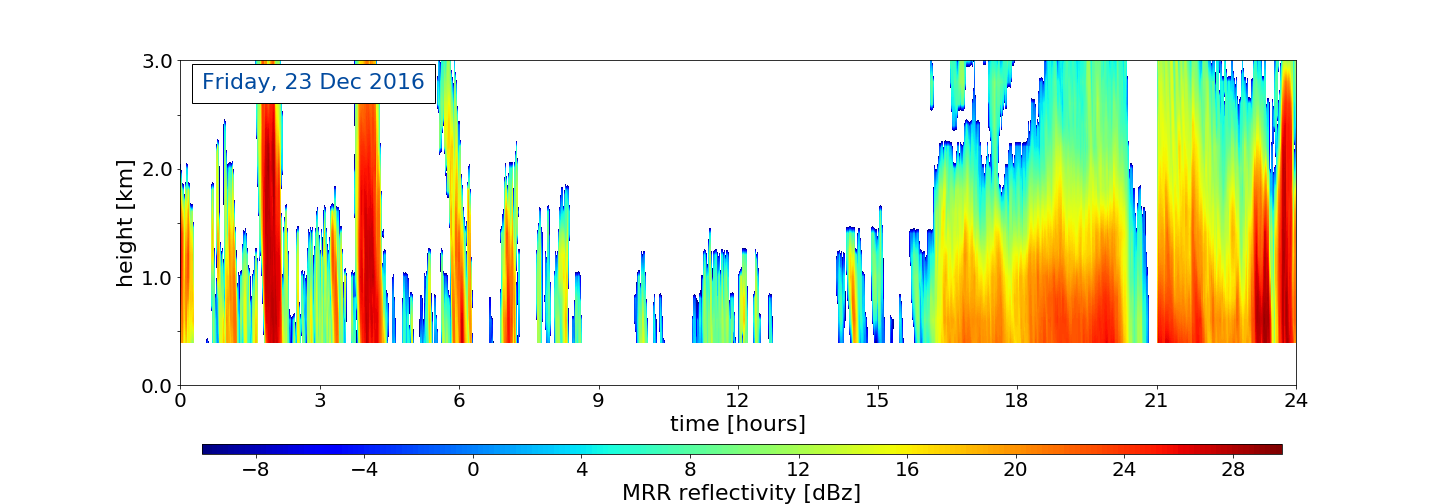
\includegraphics[trim={4.cm 2.5cm 4.5cm 1.5cm},clip,width=0.9\textwidth]{./fig_MRR_refl/MRR_20161223}
		\caption{}\label{fig:ret:refl23}
	\end{subfigure}
	% 25/12
	\begin{subfigure}[t]{\textwidth}
		\centering
		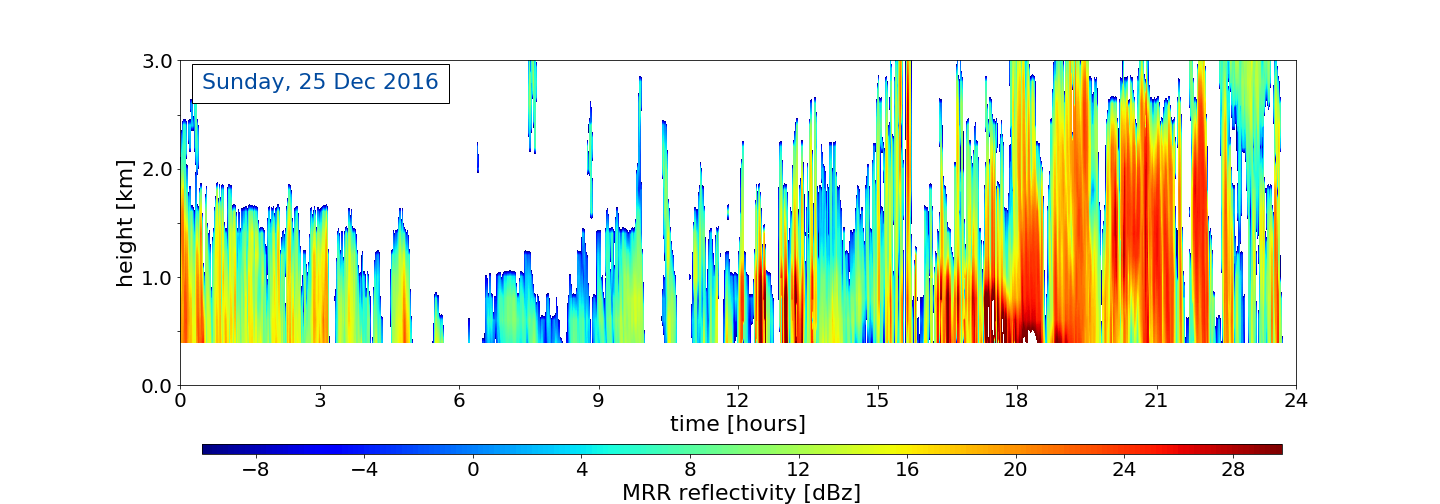
\includegraphics[trim={4.cm 2.5cm 4.5cm 1.5cm},clip,width=0.9\textwidth]{./fig_MRR_refl/MRR_20161225}
		\caption{}\label{fig:ret:refl25}
	\end{subfigure}
	% 26/12
	\begin{subfigure}[t]{\textwidth}
		\centering
		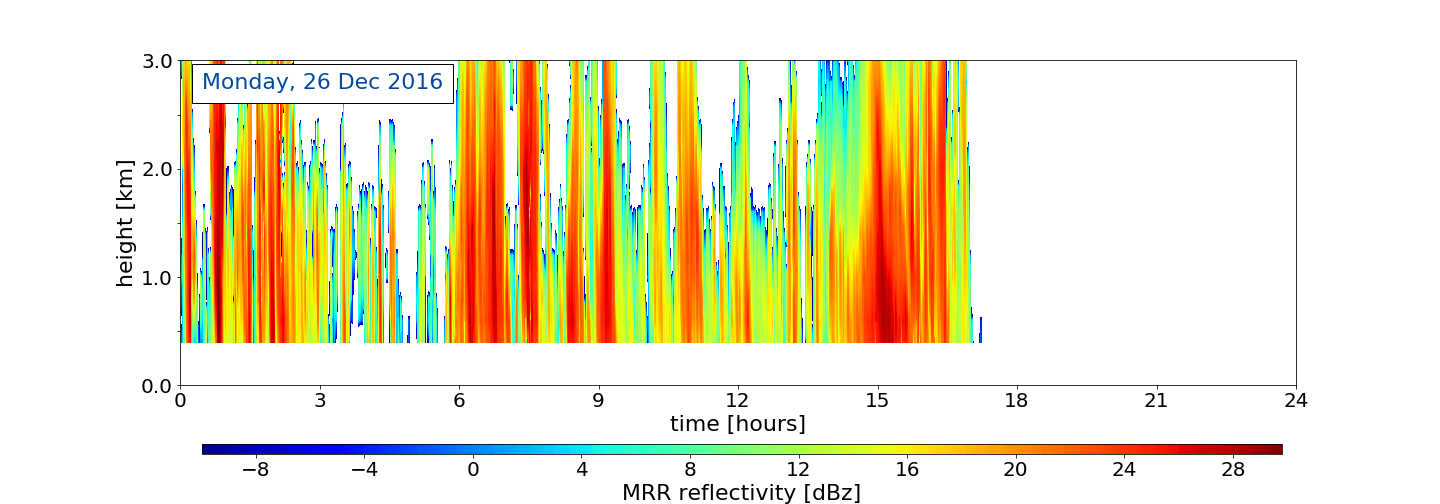
\includegraphics[trim={4.cm 2.5cm 4.5cm 1.5cm},clip,width=0.9\textwidth]{./fig_MRR_refl/MRR_20161226}
		\caption{}\label{fig:ret:refl26}
	\end{subfigure}
	% label
	\begin{subfigure}[t]{\textwidth}
		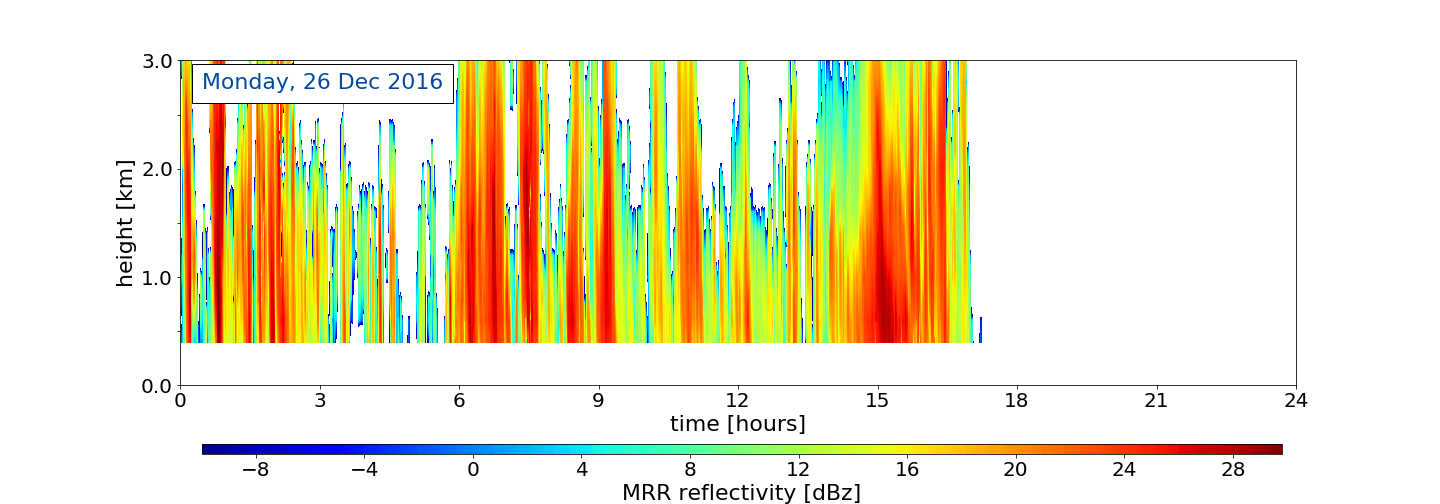
\includegraphics[trim={6.5cm 0cm 5.3cm 15.5cm},clip,width=\textwidth]{./fig_MRR_refl/MRR_20161226}
	\end{subfigure}
	\caption{MRR reflectivity for the days when a front or an occlusion passed through at Haukeliseter. \SI{}{\decibel Z} reflectivity according to the colour bar, with weaker precipitation in blue and more intense precipitation in red. \protect\subref{fig:ret:refl23}: Friday, \SI{23}{\dec}, \protect\subref{fig:ret:refl25}: Sunday, \SI{25}{\dec}, and \protect\subref{fig:ret:refl26}: Monday, \SI{26}{\dec}.}\label{fig:ret:refl}
\end{figure}
%%%%%%%%%%%%%%%%%%%%%%%%%%%%%%%%%%%%%%%%%%%%%%%%%%%%%%%%%%%%%%%%%%%%%%%%%
\noindent
Frontal boundary passages were observed at the surface several times throughout the extreme storm in December 2016. MEPS is able to predict the large scale features and related surface changes for initialisation more than \SI{24}{\hour} before (\Cref{sec:res:large_scale_sfc}). In winter 2016 three additional instruments were installed to estimate the vertical snow water content at Haukeliseter. This unique approach gives the opportunity to compare the vertical forecasts of SWC to vertical solid precipitation observations. As far as the author knows is there no study on this particular topic about the verification of vertical ensemble member prediction models with observations.
%\\
\\
\Cref{fig:ret:refl} shows the reflectivity from the MRR at Haukeliseter for \SIlist{23;25;26}{\dec}. Passages of occluded fronts and a warm sector were observed on \SIlist{23;26;25}{\dec}, respectively. \Cref{fig:ret:refl26} presents only values until \SI{17}{\UTC}, because of the temperature change and hence a precipitation shift followed liquid drops freezing on the MRR dish and the signal got attenuated. 
\\
The transit of the boundary is shown in \Cref{fig:ret:refl} by the more consistent structure of a storm with higher reflectivity values. 
While on \SIlist{23;26}{\dec} the reflectivity did not pass values larger than \SI{28}{\decibel Z} shows \Cref{fig:ret:refl25} high reflectivity values larger than \SI{30}{\decibel Z} (compare for approximation \Cref{tab:ref_values}). These high values indicate the observation of possible liquid precipitation. Images from the MASC were able to verify observed liquid drops during \SIrange{12}{21}{\UTC} (\Cref{fig:res:obs_masc}). 
\\
On \SI{23}{\dec} allow the surface observations to assume that the occluded front passed through between \SIrange{12}{21}{\UTC} (\Cref{fig:res:sfc_pres23}, \subref{fig:res:sfc_temp23}, \subref{fig:res:sfc_wd23}). The vertical observations at Haukeliseter show intense reflectivity and therefore more intense precipitation after \SI{16}{\UTC} (\Cref{fig:ret:refl23}). Another occlusion passed through on \SI{26}{\dec} shortly before \SI{15}{\UTC} which lasted until \SI{21}{\UTC} indicated by a more consistent storm structure in \Cref{fig:ret:refl26} around \SI{15}{\UTC}. The high reflectivity on both days shows the passage of the occlusion and the associated precipitation. The wind on \SI{23}{\dec} was from the south, upslope (\Cref{fig:res:sfc_wd23}, \Cref{fig:site:kartverket}) which led to a more consistent storm structure. On \SI{25}{\dec} indicate \Cref{fig:res:sfc_wd25} and \subref{fig:res:sfc_ws25} strong wind observations from the west which led to a consistent, but shorter storm structure in \Cref{fig:ret:refl25} at \SI{15}{\UTC}. The orographic influenced wind and therefore a possible relation to the precipitation will be further assessed in \Cref{sec:res:oro_infl}. 
\\
\\
\Cref{fig:SWC} presents the reflectivity from the MRR and the snow water content retrieved from the reflectivity as well as the \SI{48}{\hour} forecast values. Minutely MRR reflectivity and retrieved snow water content can be seen in \Cref{fig:SWC:ret_22}, \subref{fig:SWC:ret_23}, \subref{fig:SWC:ret_25}, and \subref{fig:SWC:ret_26}. \Cref{fig:SWC_EM:22}, \subref{fig:SWC_EM:23}, \subref{fig:SWC_EM:25}, \subref{fig:SWC_EM:26} show in the upper panel the hourly averaged values from the retrieved SWC and in the lower panel the ensemble mean of the instantaneous forecast values every hour over all ensemble member.   
Three hourly averaged retrieved values are then presented in the upper panel of \Cref{fig:SWC3h:22}, \subref{fig:SWC3h:23}, \subref{fig:SWC3h:25}, and \subref{fig:SWC3h:26}, the lower panel are the ensemble mean forecast values every three hours.
\\
\Cref{fig:SWC_EM:23} (lower panel) shows the one hourly averaged forecast values over all ensemble members, neglecting not existing values. Initialisations less than \SI{24}{\hour} before the event predict the consistent retrieved snowfall after \SI{16}{\UTC} (\Cref{fig:SWC:ret_23}, lower panel and \Cref{fig:SWC_EM:23}, upper panel). Even the three hourly averaged forecast values show a response on the occurrence of the storm (\Cref{fig:SWC3h:23}, lower panel). 
The duration of the passage is between \SIrange{16}{23}{\UTC} because of the longer time span is the prediction system able to estimate the snow water content. Forecasts initialised \SI{48}{\hour} prior predict also the consistent storm structure and therefore the passage of the front (\Cref{fig:SWC_EM:22}, \subref{fig:SWC3h:22}). 
\\
In general, is the forecasted instantaneous snow water content amount weaker than the retrieved values for predications on \SI{23}{\dec}. Hourly averages, only using the deterministic forecast and the first ensemble member show no occurrence of the occlusion passage on either day (\Cref{fig:SWC1h:22}, \subref{fig:SWC1h:23}, \subref{fig:SWC1h:25}, \subref{fig:SWC1h:26}). The variation of each ensemble member initialised on the respective day are given in \Cref{fig:EM09}. In \Cref{fig:EM09_22} is the prediction for the occlusion passage quite weak. 
%%%%%%%%% image SWC retrieval MEPS 22 %%%%%%%%%%%%%%
\begin{figure}[H]
	\centering
	% 23/12
	\begin{subfigure}[t]{\textwidth}
		\centering
		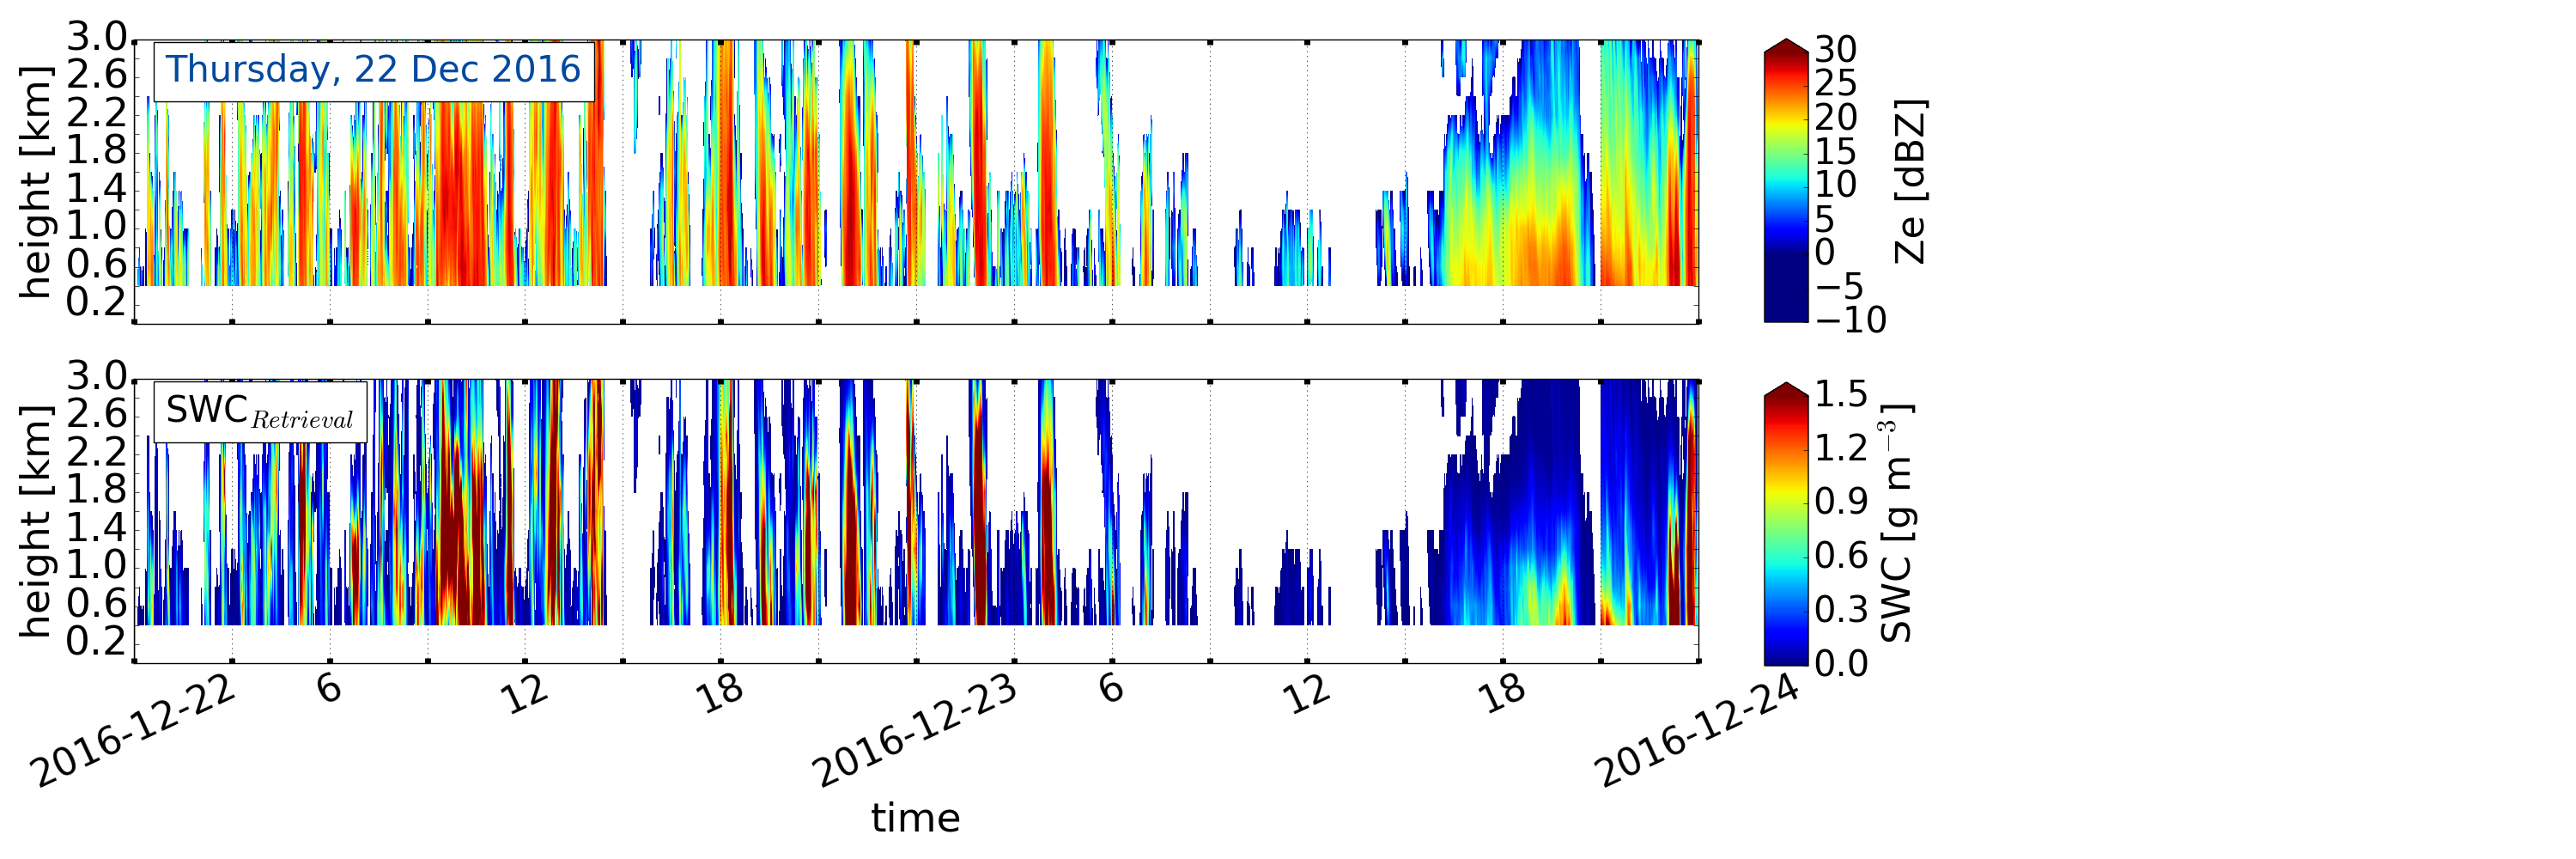
\includegraphics[trim={0.cm 2.2cm 19.cm 0.5cm},clip,width=0.9\textwidth]{./fig_obs_ret/20161222}
		\caption{}\label{fig:SWC:ret_22}
	\end{subfigure}
	% EM
	\begin{subfigure}[t]{\textwidth}
		\centering
		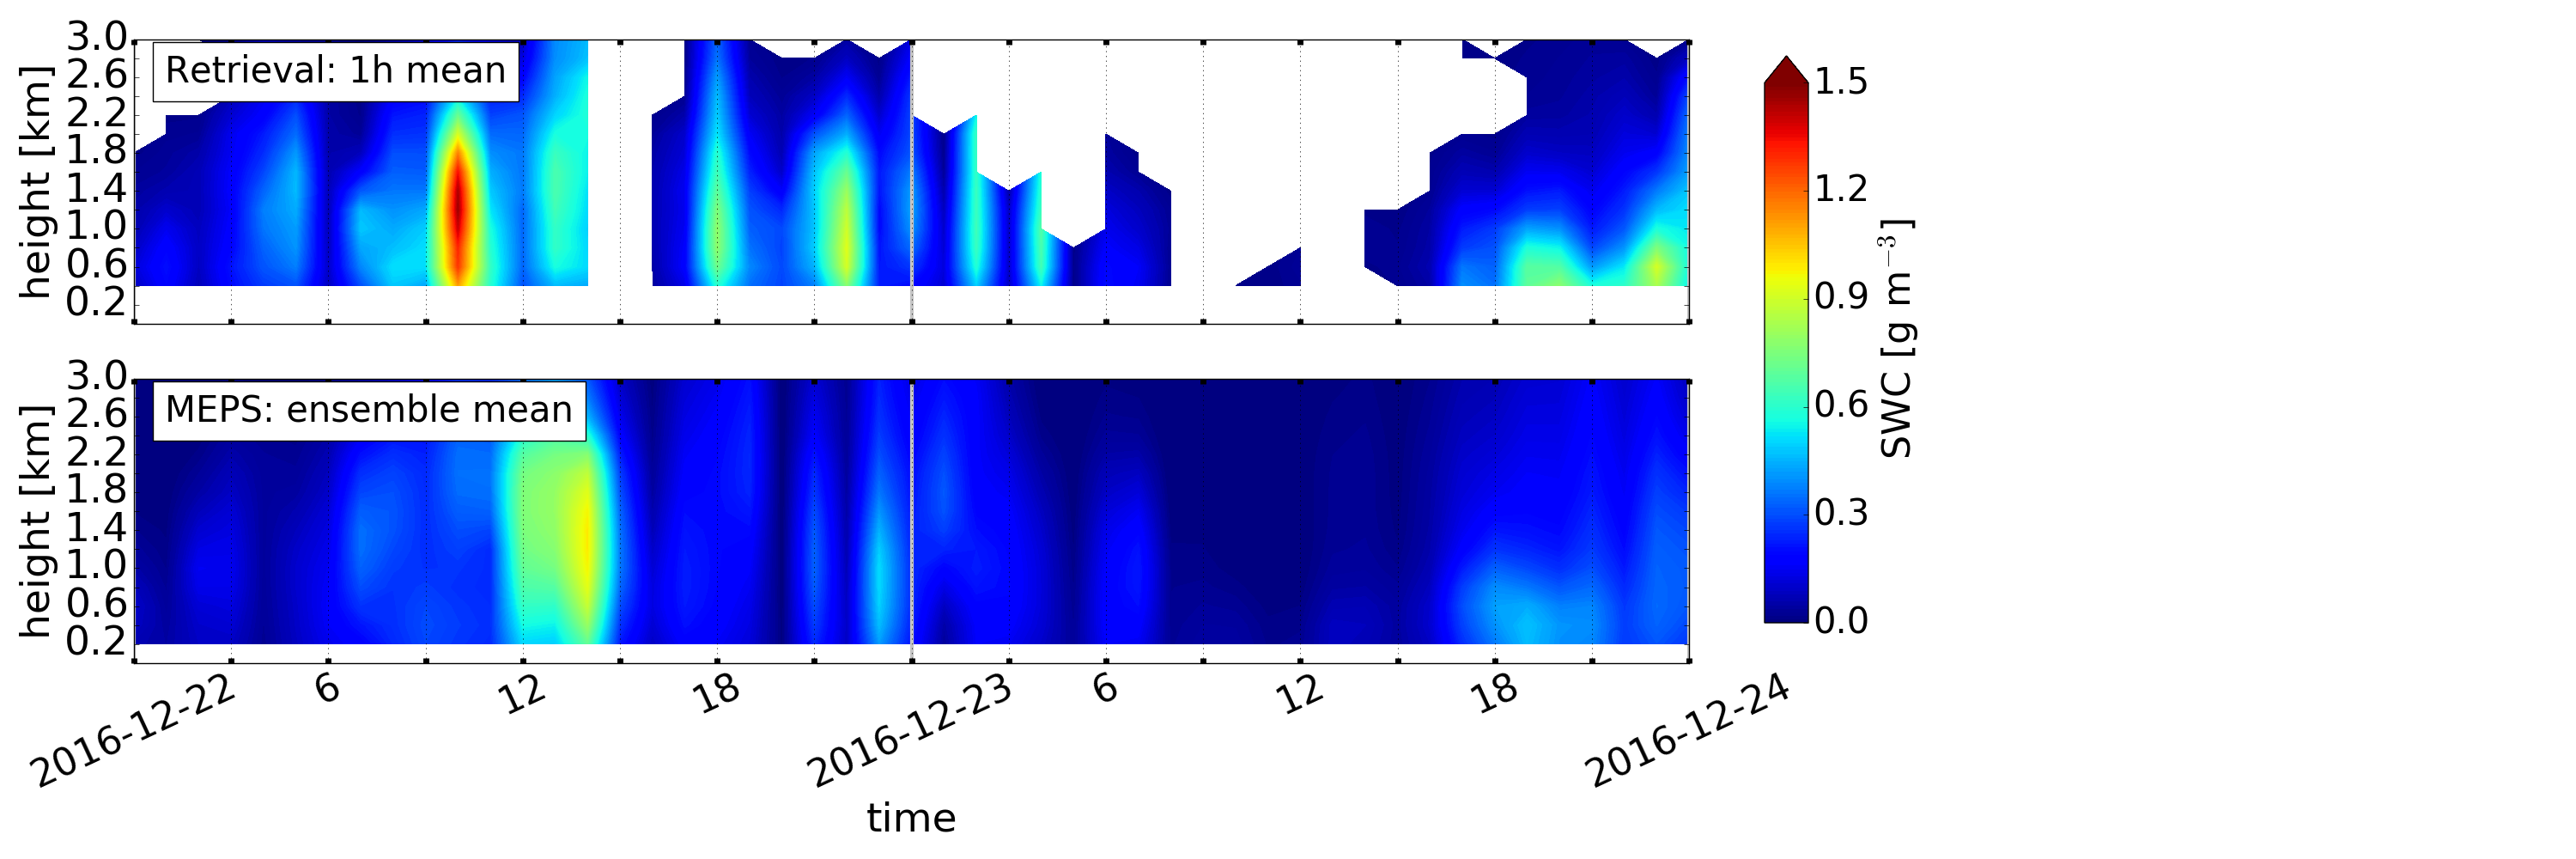
\includegraphics[trim={0.cm 2.2cm 19.cm 0.5cm},clip,width=0.9\textwidth]{./fig_vert_SWC_EM/20161222}
		\caption{}\label{fig:SWC_EM:22}
	\end{subfigure}
	% 3h
	\begin{subfigure}[t]{\textwidth}
		\centering
		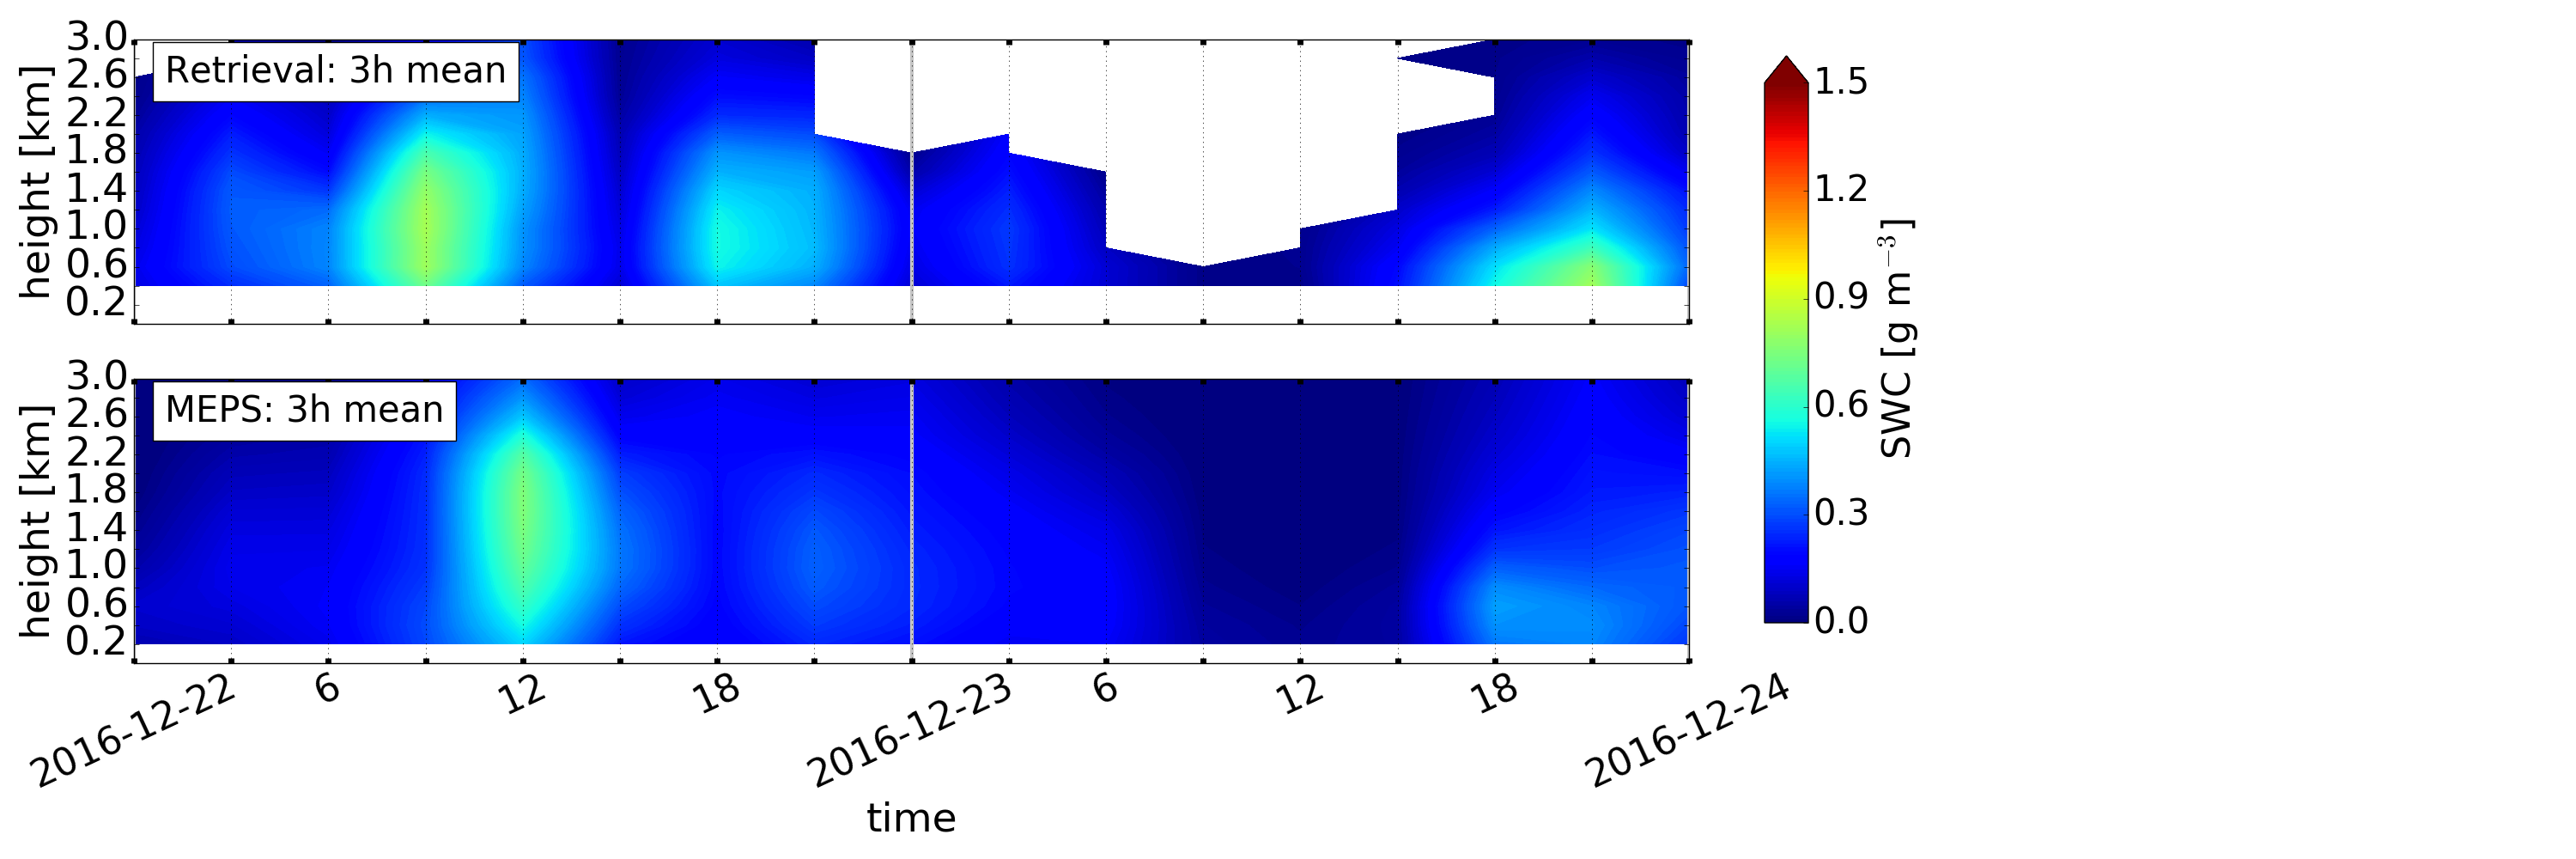
\includegraphics[trim={0.cm 0.8cm 19.cm 0.5cm},clip,width=0.9\textwidth]{./fig_vert_SWC_3h/20161222}
		\caption{}\label{fig:SWC3h:22}
	\end{subfigure}
	\caption{Initialisation \SIlist{22;23;25;26}{\dec} \SI{0}{\UTC}. 
		(\protect\subref{fig:SWC:ret_22},\protect\subref{fig:SWC:ret_23}, \protect\subref{fig:SWC:ret_25}, \protect\subref{fig:SWC:ret_26}) Upper panel: MRR reflectivity for \SI{48}{\hour}, lower panel minutely retrieved SWC. 
		(\protect\subref{fig:SWC_EM:22}, \protect\subref{fig:SWC_EM:23}, \protect\subref{fig:SWC_EM:25}, \protect\subref{fig:SWC_EM:26}) Upper panel: hourly averaged retrieved SWC, lower panel instantaneous hourly averaged forecast of all ensemble member SWC, neglecting missing values. 
		(\protect\subref{fig:SWC3h:22}, \protect\subref{fig:SWC3h:23}, \protect\subref{fig:SWC3h:25}, \protect\subref{fig:SWC3h:26}) Upper panel three hourly averaged retrieved SWC, lower panel instantaneous three hourly averaged forecast of all ensemble member SWC.   }\label{fig:ret:SWC}
\end{figure}
%%%%%%%%% image SWC retrieval MEPS 23 %%%%%%%%%%%%%%
\begin{figure}[H]\ContinuedFloat
	\centering
	% 23/12
	\begin{subfigure}[t]{\textwidth}
		\centering
		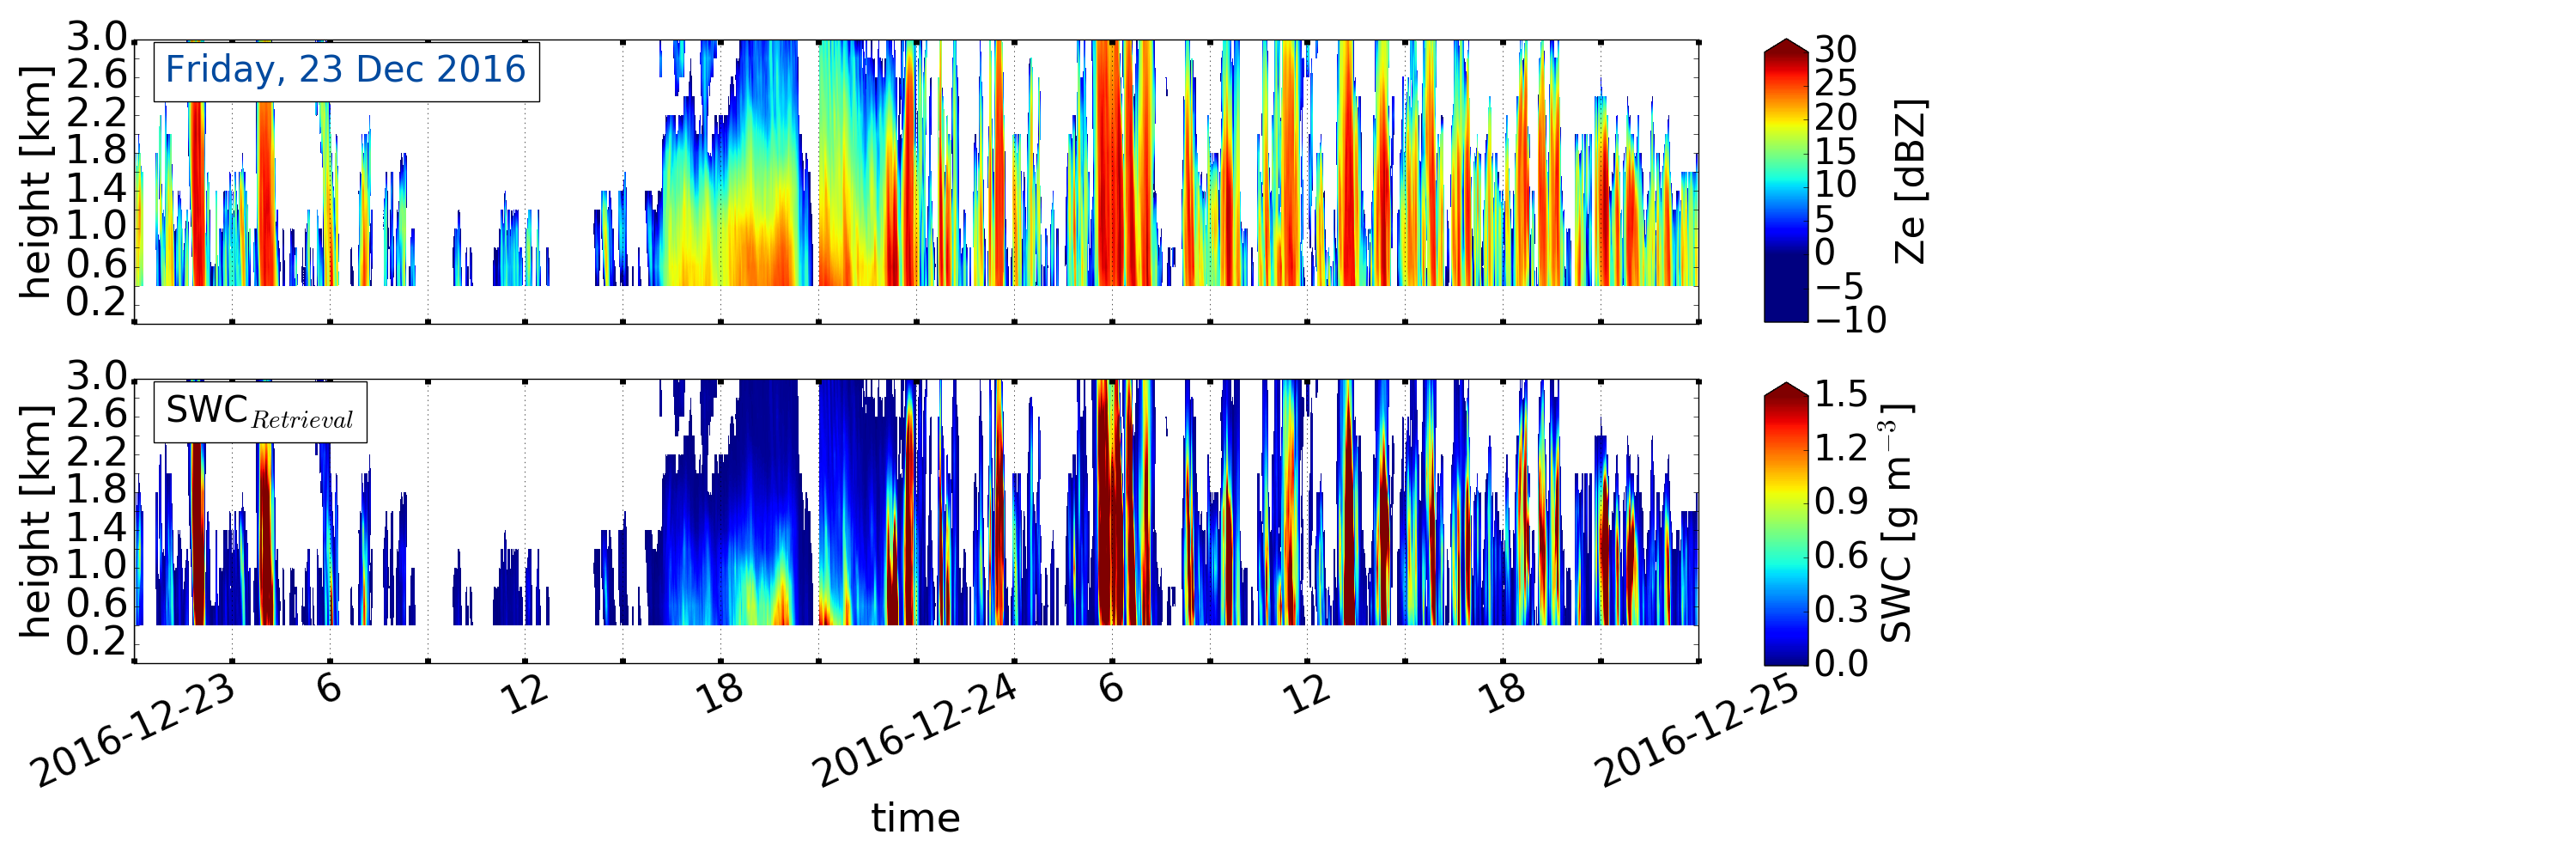
\includegraphics[trim={0.cm 2.2cm 19.cm 0.5cm},clip,width=0.9\textwidth]{./fig_obs_ret/20161223}
		\caption{}\label{fig:SWC:ret_23}
	\end{subfigure}
	% EM
	\begin{subfigure}[t]{\textwidth}
		\centering
		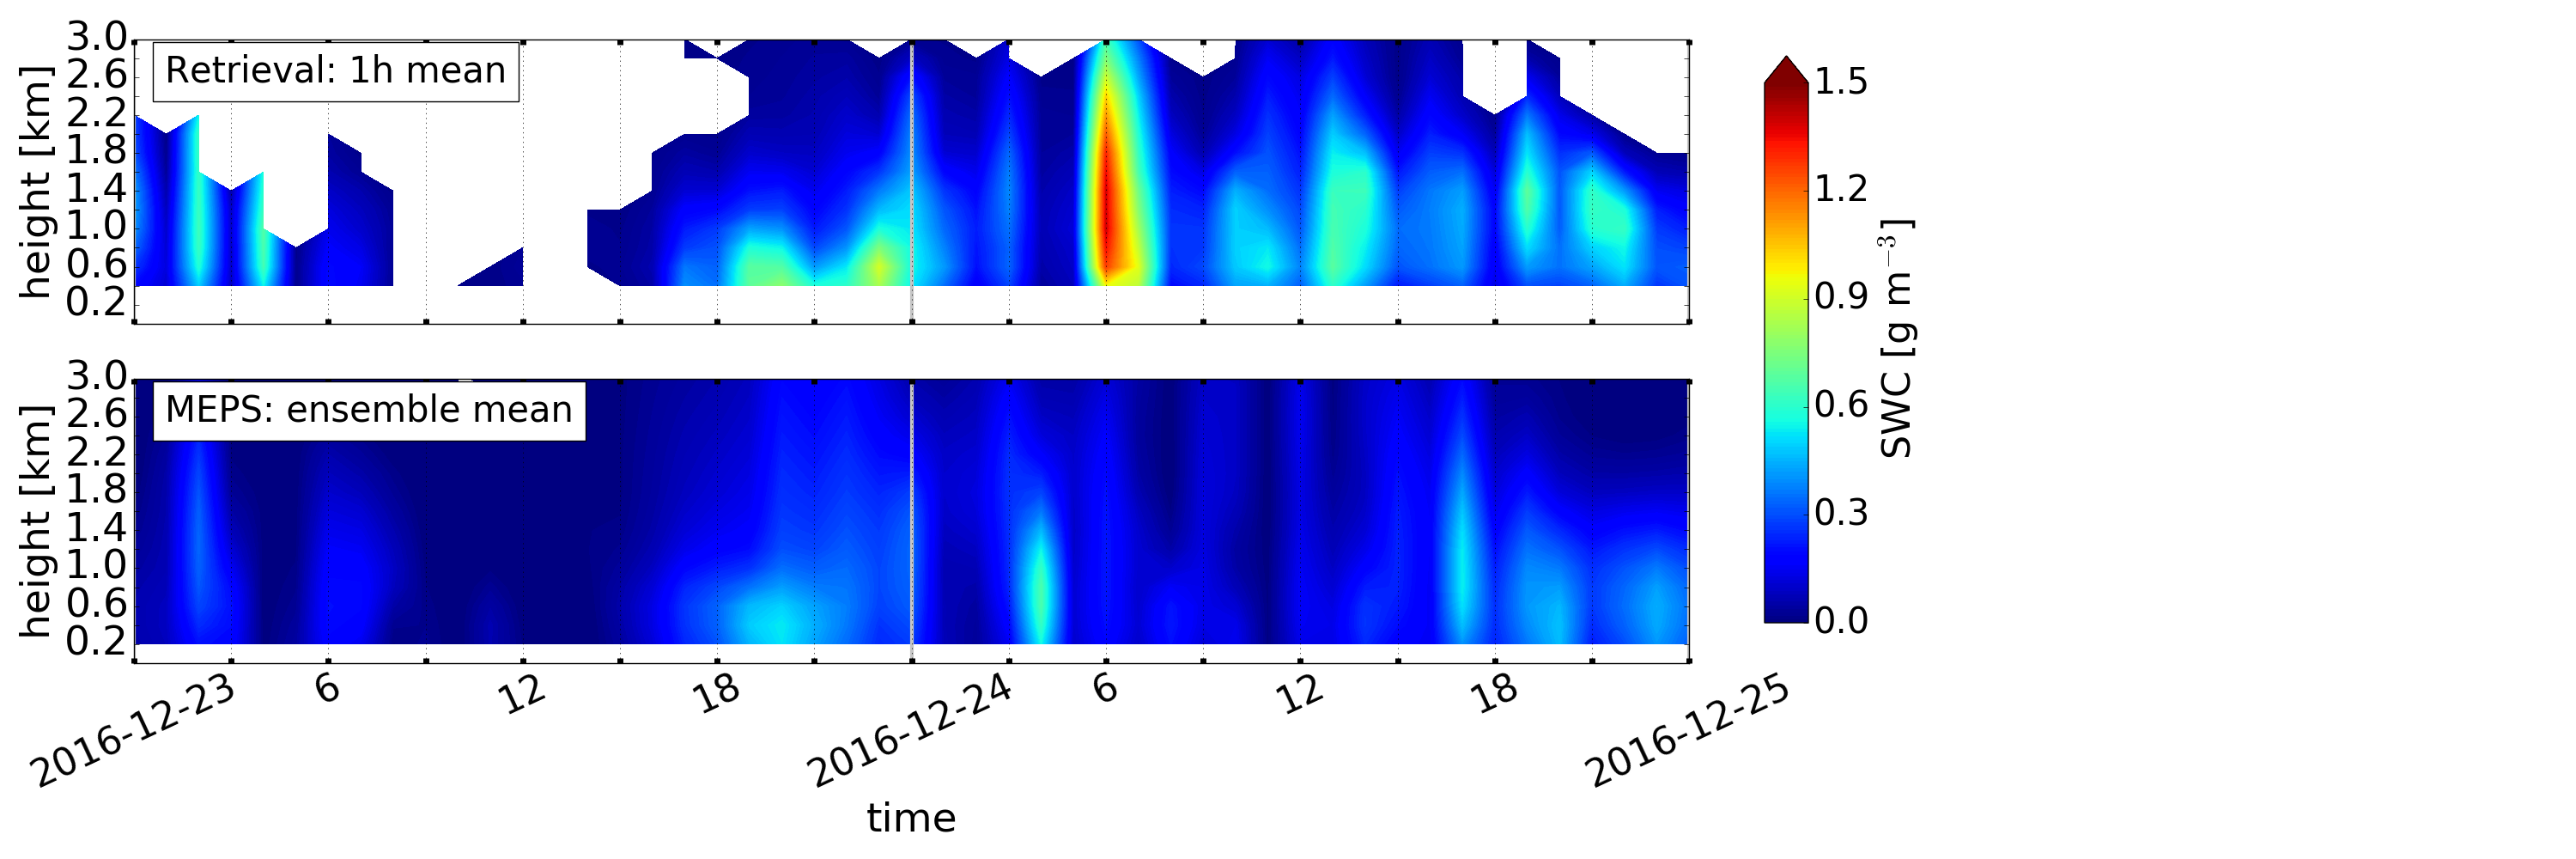
\includegraphics[trim={0.cm 2.2cm 19.cm 0.5cm},clip,width=0.9\textwidth]{./fig_vert_SWC_EM/20161223}
		\caption{}\label{fig:SWC_EM:23}
	\end{subfigure}
	% 3h
	\begin{subfigure}[t]{\textwidth}
		\centering
		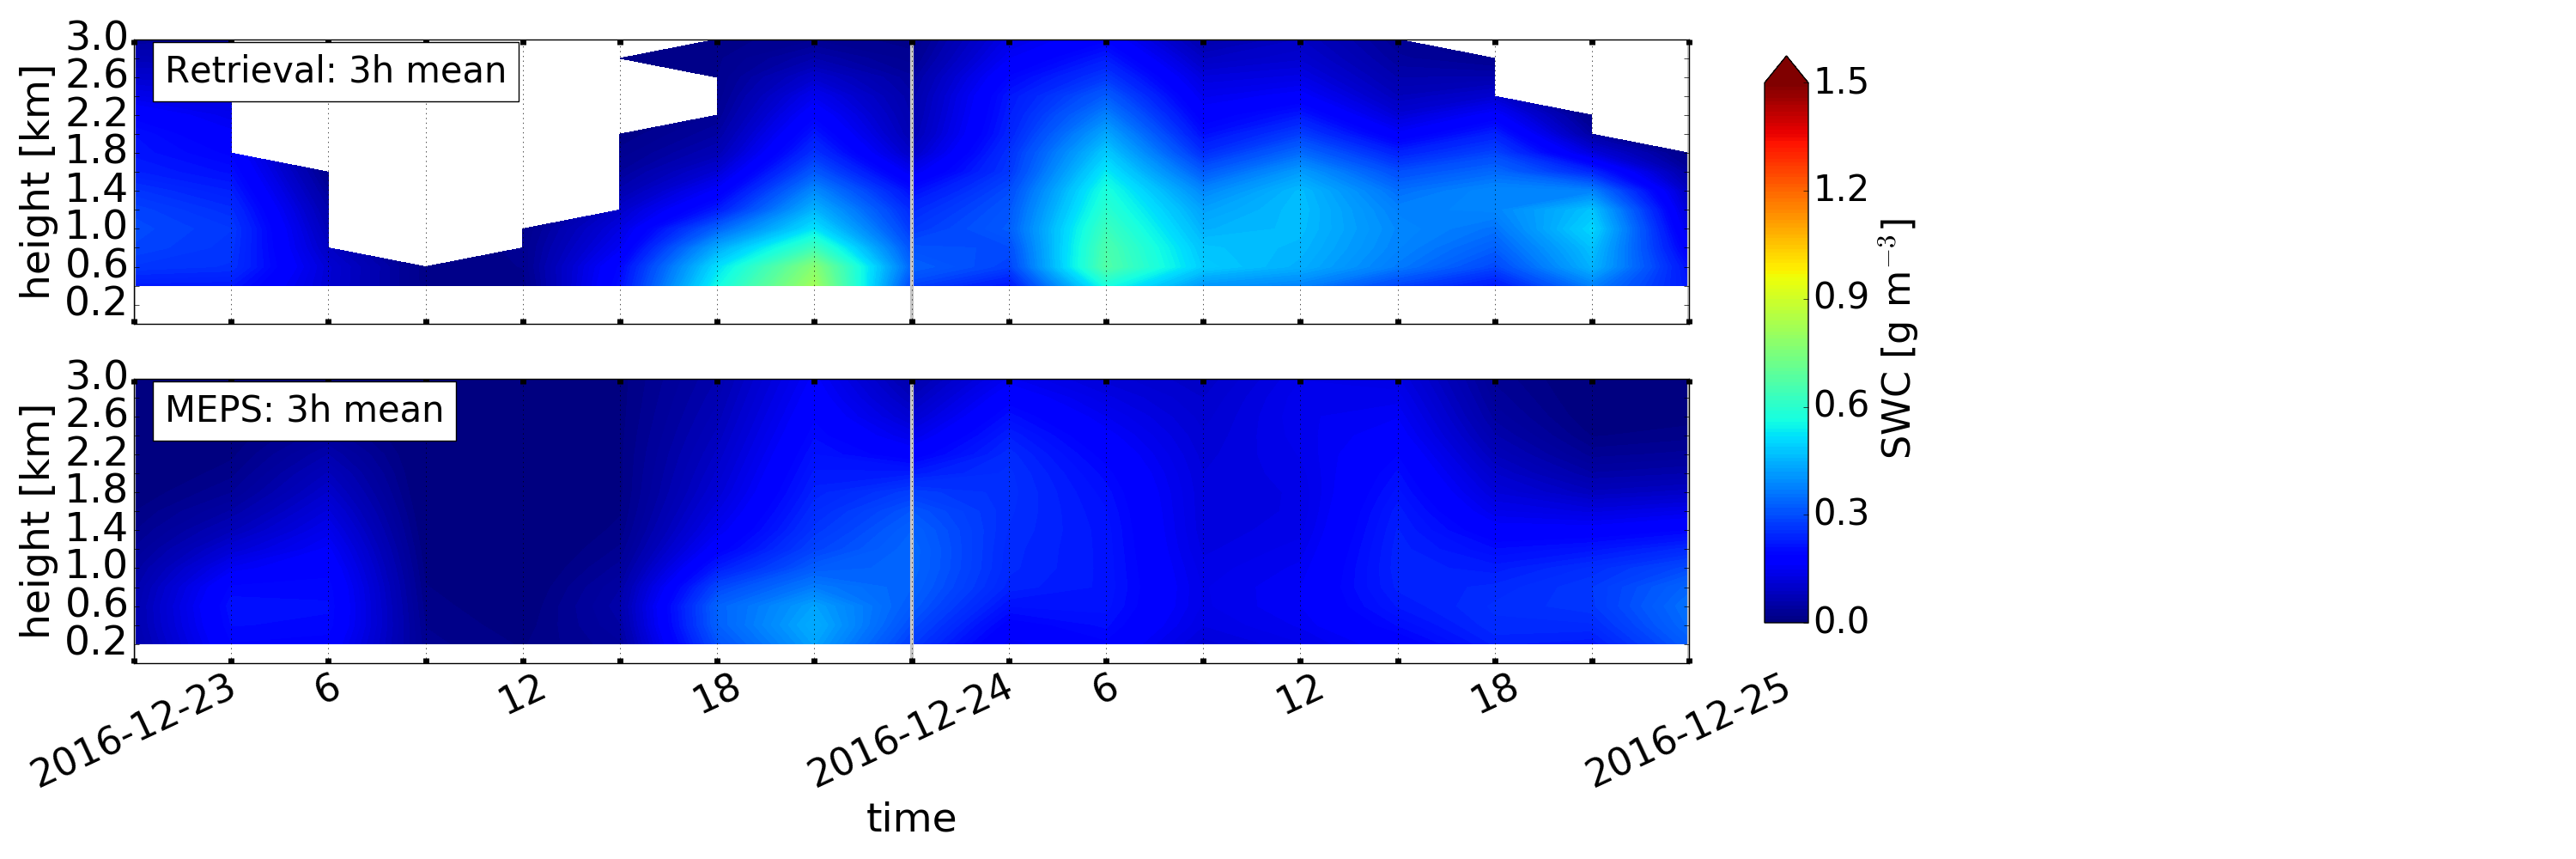
\includegraphics[trim={0.cm 0.8cm 19.cm 0.5cm},clip,width=0.9\textwidth]{./fig_vert_SWC_3h/20161223}
		\caption{}\label{fig:SWC3h:23}
	\end{subfigure}
	\caption{\textit{(Continued from previous page.)} Initialisation \SI{23}{\dec}.}
\end{figure}
%%%%%%%%% image SWC retrieval MEPS 25 %%%%%%%%%%%%%%
\begin{figure}[H]\ContinuedFloat
	\centering
	% 25/12
	\begin{subfigure}[t]{\textwidth}
		\centering
		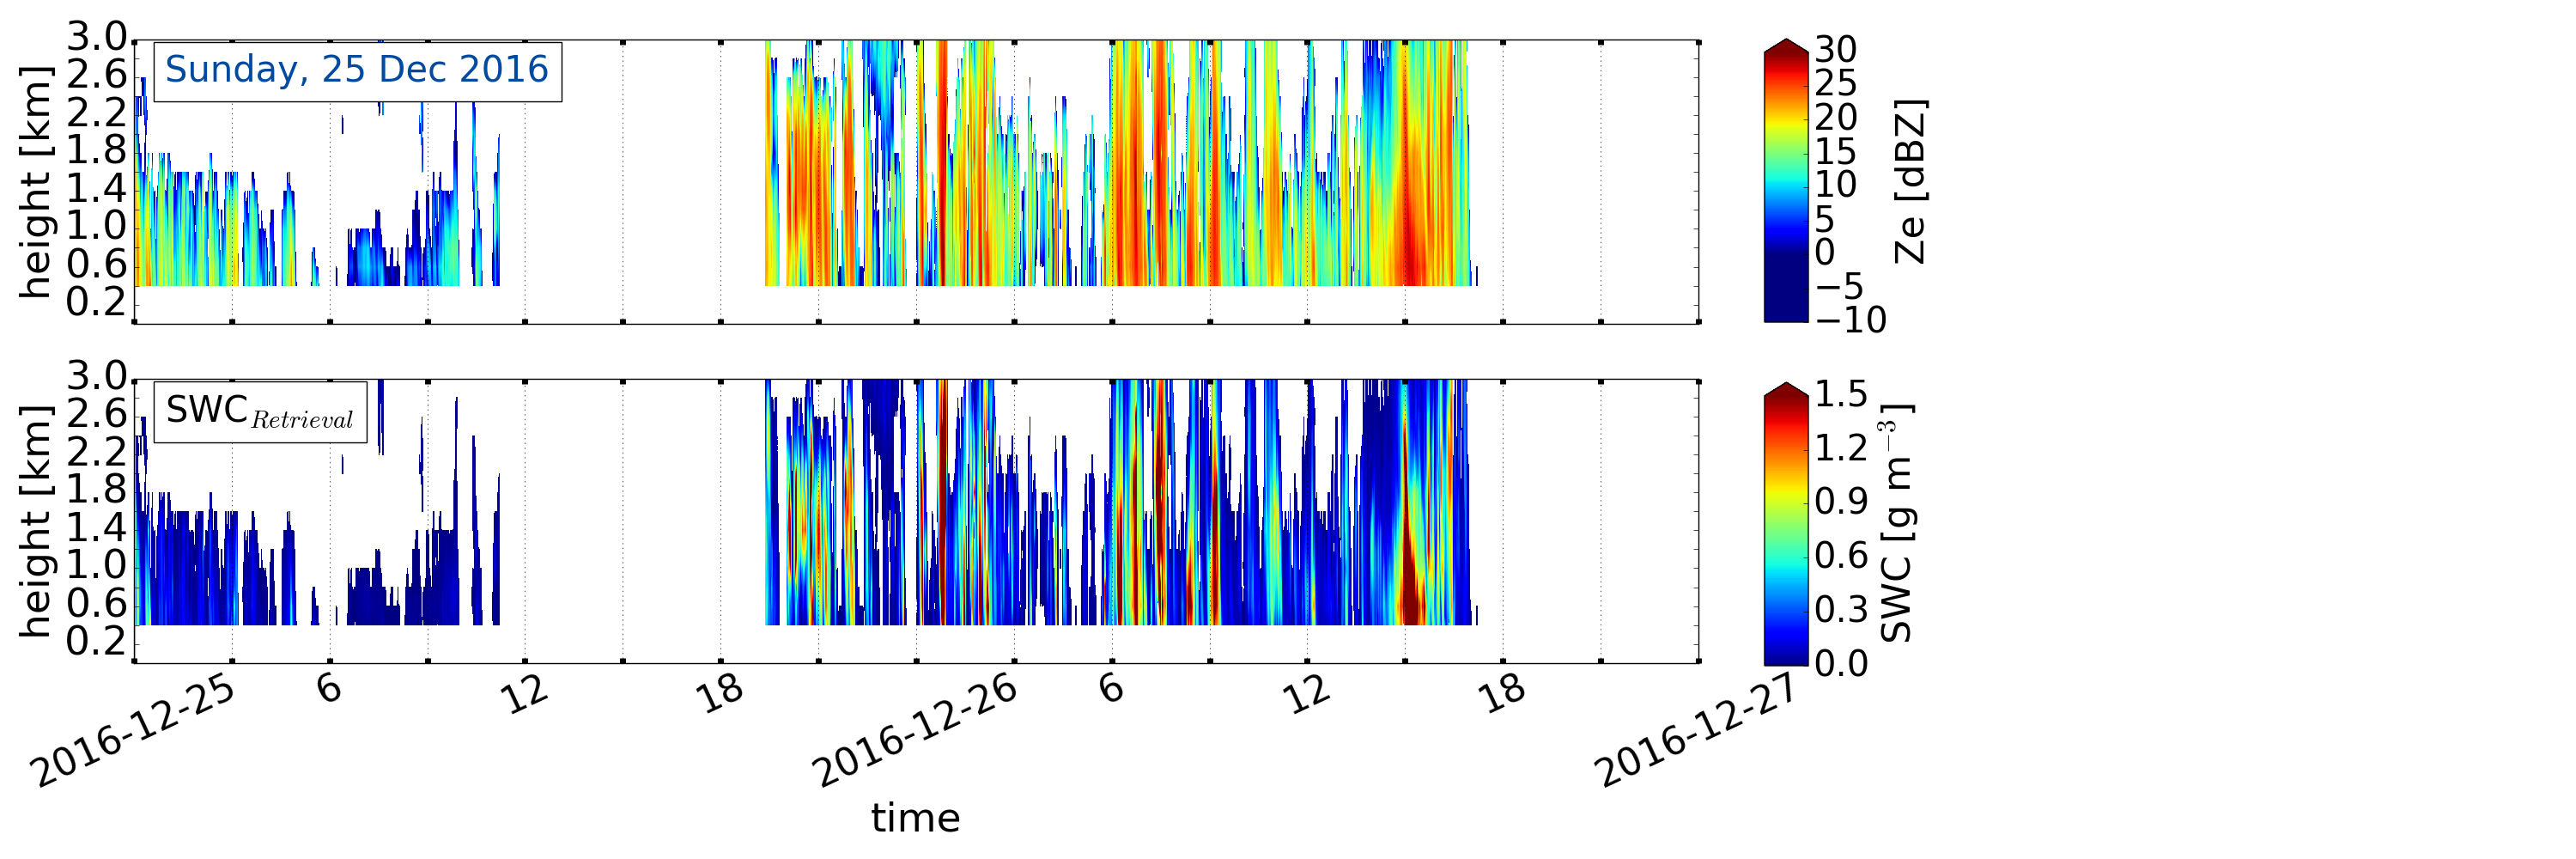
\includegraphics[trim={0.cm 2.2cm 19.cm 0.5cm},clip,width=0.9\textwidth]{./fig_obs_ret/20161225}
		\caption{}\label{fig:SWC:ret_25}
	\end{subfigure}
	% EM
	\begin{subfigure}[t]{\textwidth}
		\centering
		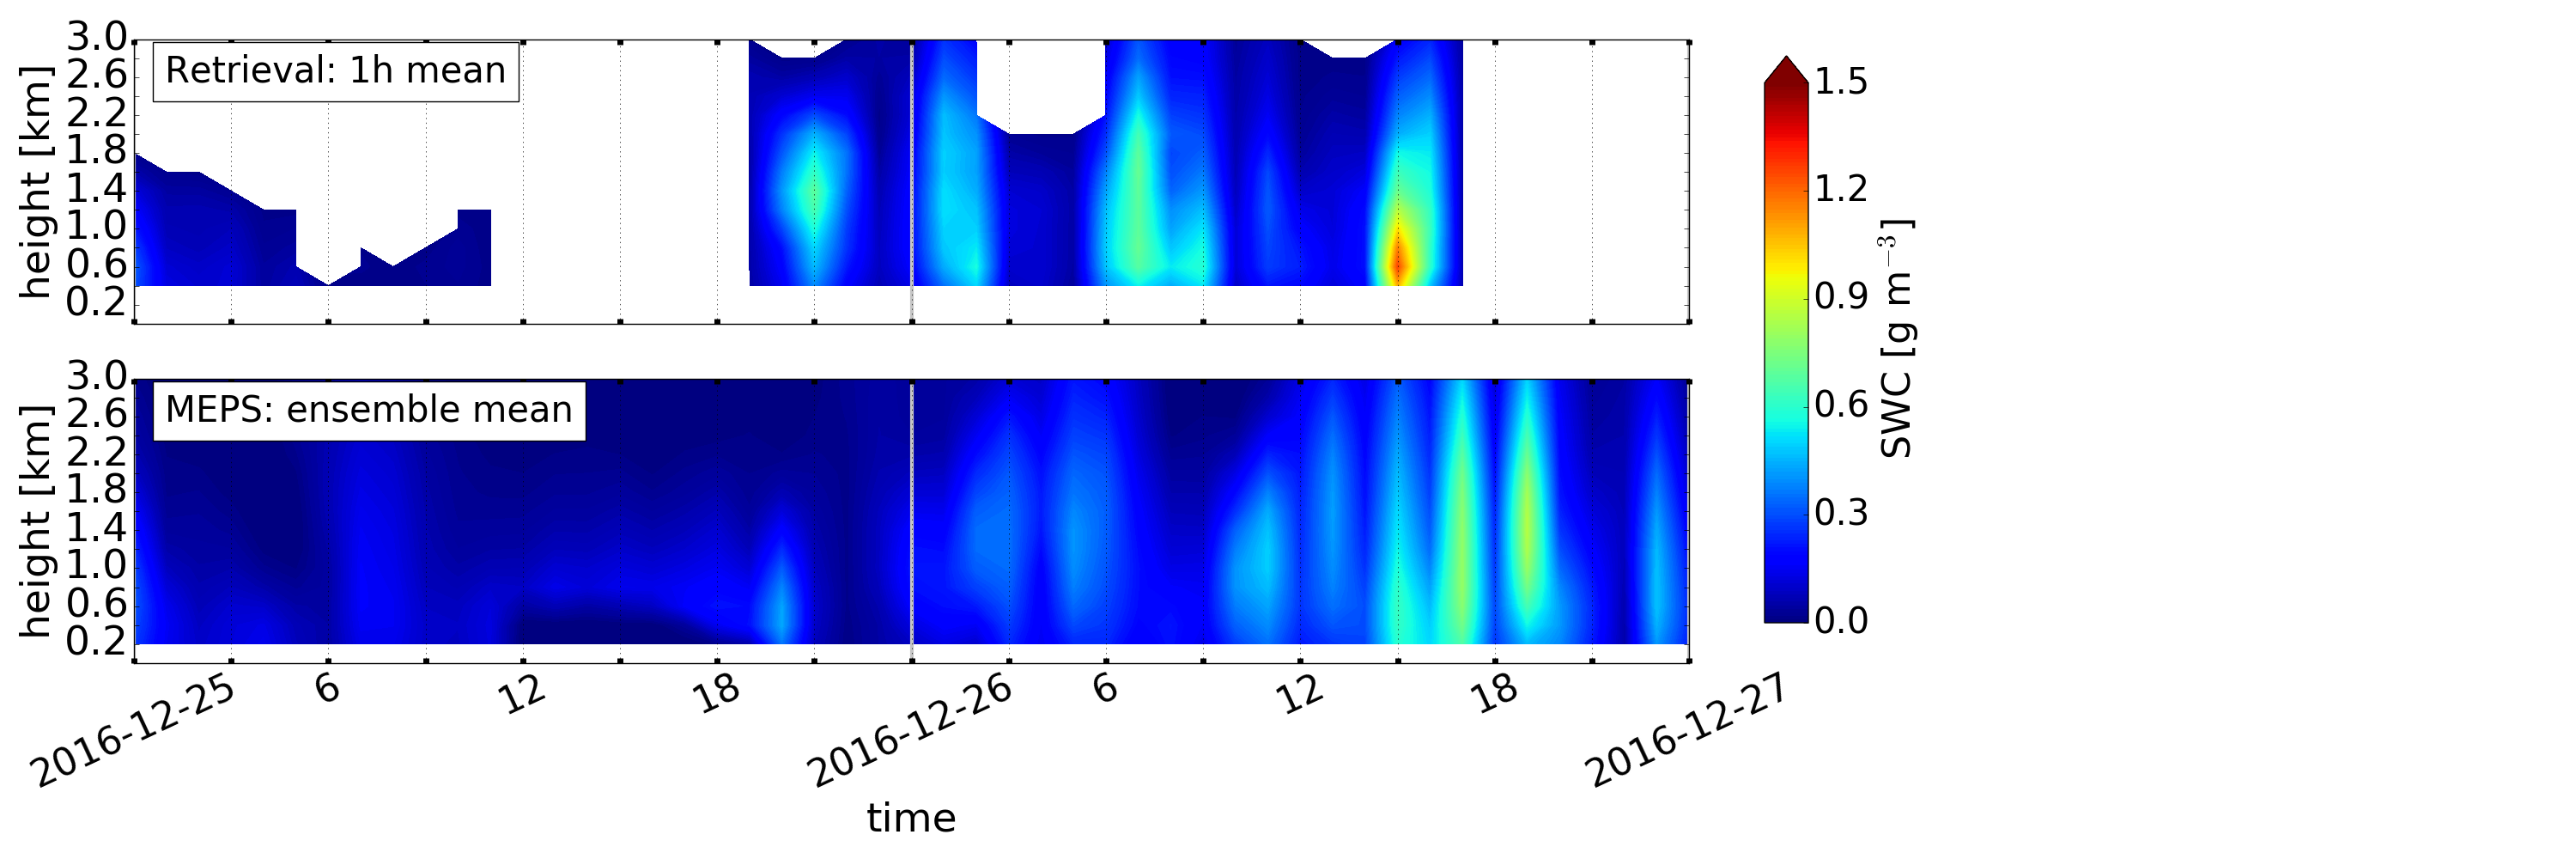
\includegraphics[trim={0.cm 2.2cm 19.cm 0.5cm},clip,width=0.9\textwidth]{./fig_vert_SWC_EM/20161225}
		\caption{}\label{fig:SWC_EM:25}
	\end{subfigure}
	% 3h
	\begin{subfigure}[t]{\textwidth}
		\centering
		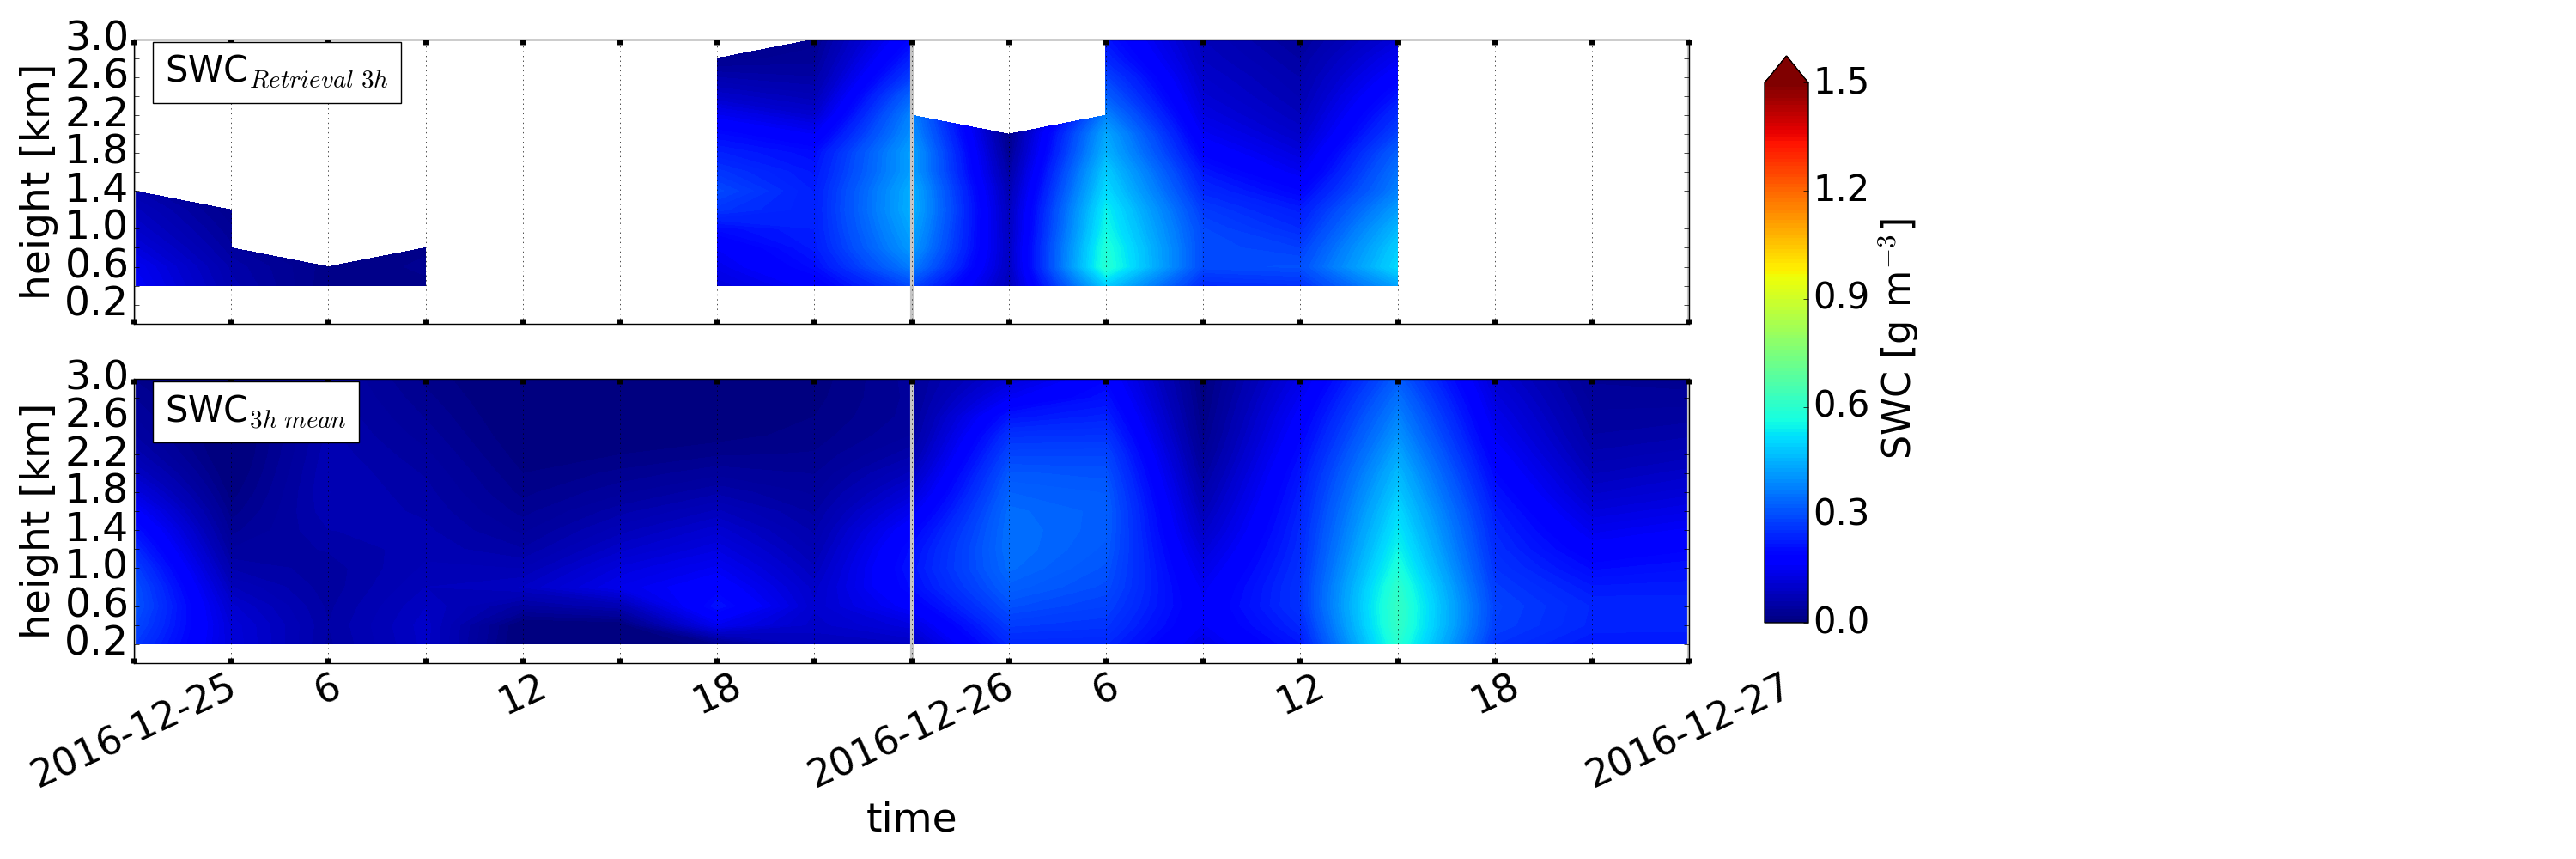
\includegraphics[trim={0.cm 0.8cm 19.cm 0.5cm},clip,width=0.9\textwidth]{./fig_vert_SWC_3h/20161225}
		\caption{}\label{fig:SWC3h:25}
	\end{subfigure}
	\caption{\textit{(Continued from previous page.)} Initialisation \SI{25}{\dec}.}
\end{figure}
%%%%%%%%% image SWC retrieval MEPS 26 %%%%%%%%%%%%%%
\begin{figure}[H]\ContinuedFloat
	\centering
	% 25/12
	\begin{subfigure}[t]{\textwidth}
		\centering
		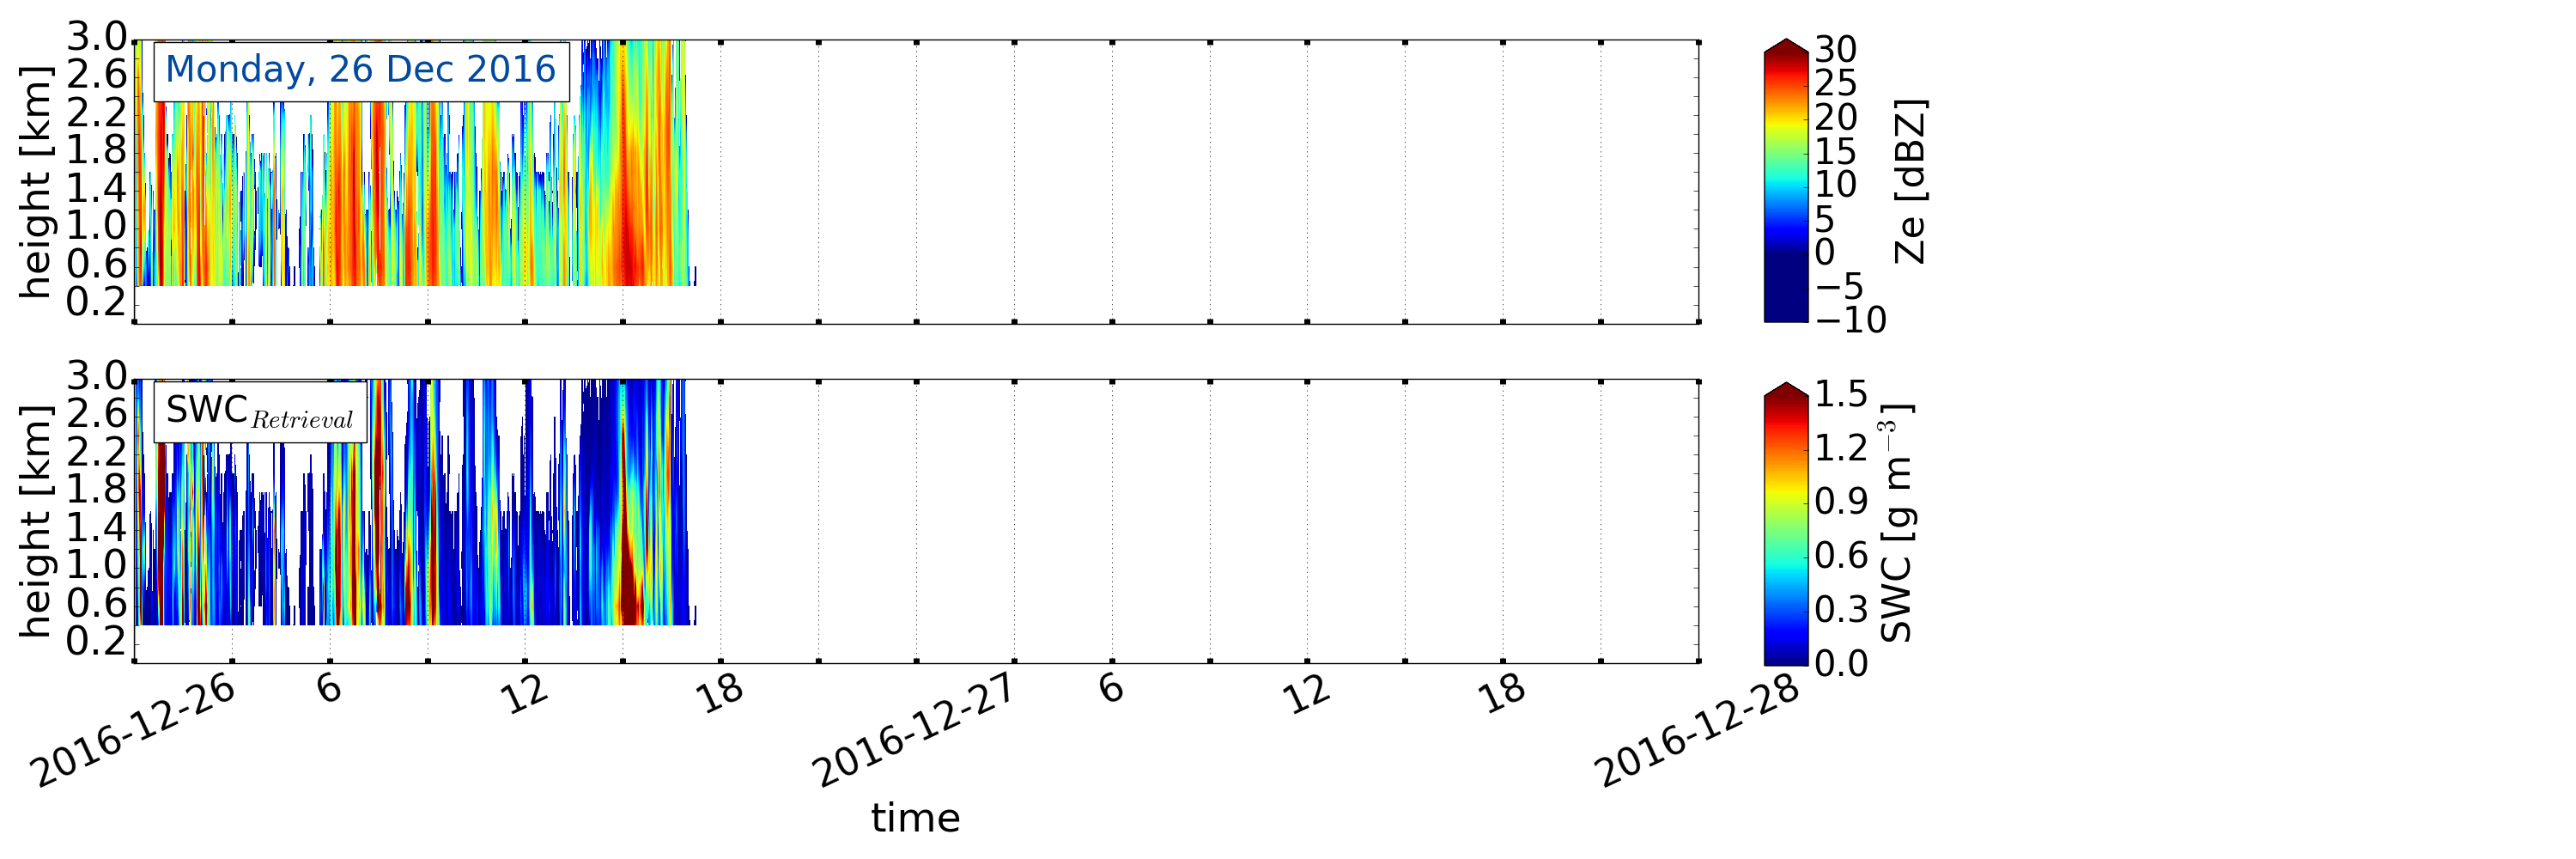
\includegraphics[trim={0.cm 2.2cm 19.cm 0.5cm},clip,width=0.9\textwidth]{./fig_obs_ret/20161226}
		\caption{}\label{fig:SWC:ret_26}
	\end{subfigure}
	% EM
	\begin{subfigure}[t]{\textwidth}
		\centering
		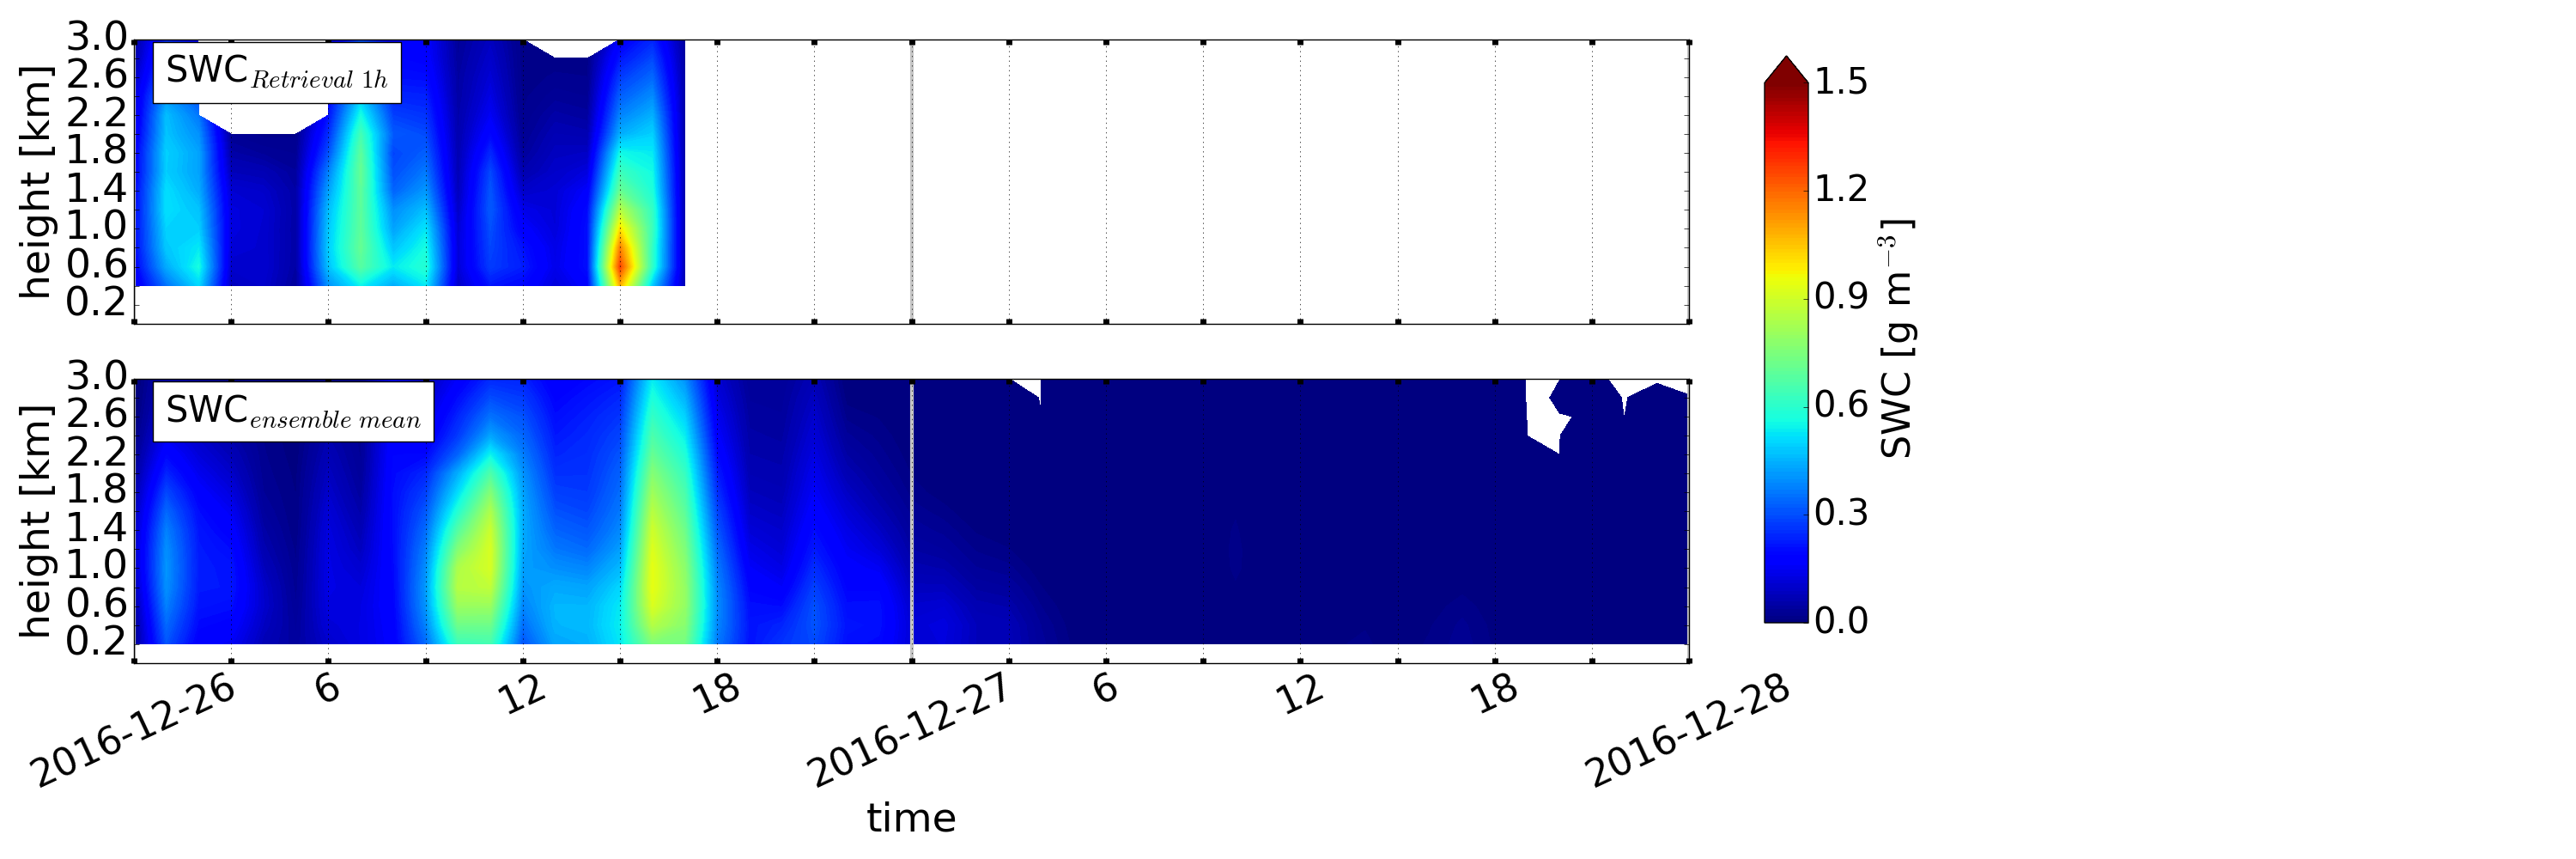
\includegraphics[trim={0.cm 2.2cm 19.cm 0.5cm},clip,width=0.9\textwidth]{./fig_vert_SWC_EM/20161226}
		\caption{}\label{fig:SWC_EM:26}
	\end{subfigure}
	% 3h
	\begin{subfigure}[t]{\textwidth}
		\centering
		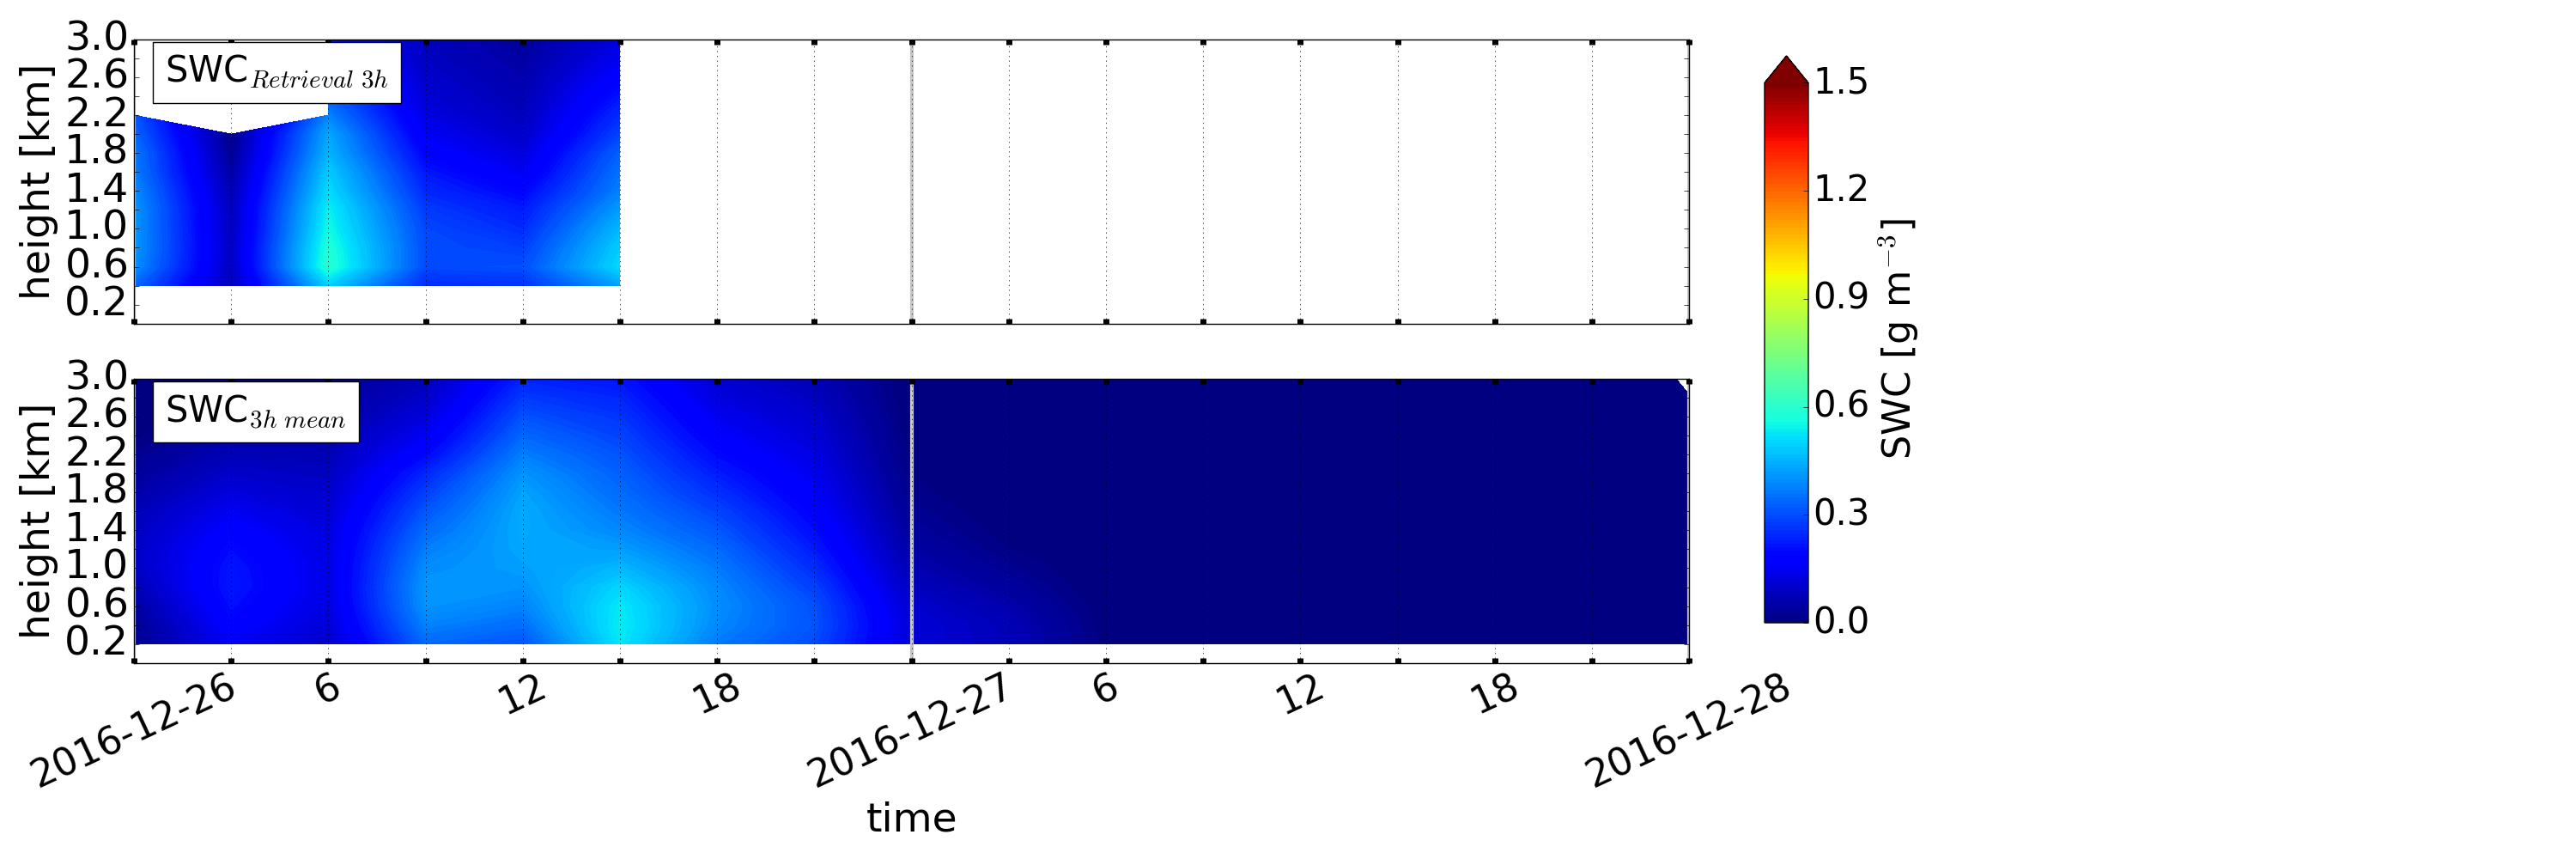
\includegraphics[trim={0.cm 0.8cm 19.cm 0.5cm},clip,width=0.9\textwidth]{./fig_vert_SWC_3h/20161226}
		\caption{}\label{fig:SWC3h:26}
	\end{subfigure}
	\caption{\textit{(Continued from previous page.)} Initialisation \SI{26}{\dec}.}
\end{figure}
%%%%%%%%%%%%%%%%%%%%%%%%%%%%%%%%%%%%%%%%%%%%%%%%%%%%%%%%%%%%%%%%%%%%%%%%%
\noindent
It shows also on \SI{23}{\dec} the first perturbed ensemble member does not exist and hence little snow water content is predicted for the ensemble means. 
A comparison with \SIlist{25;26}{\dec} shows the same result. Not much more snow water content is predicted when using the instantaneous values from the deterministic and first perturbed forecast (\Cref{fig:SWC1h:25}, \subref{fig:SWC1h:26}). 
\\ 
On \SI{26}{\dec} when the passage of the occlusion is predicted, the three-hourly instantaneous SWC (\Cref{fig:SWC3h:26}) as well as the average of all ensemble members (\Cref{fig:SWC_EM:26}) predict the frontal passage. 
Already initialisations \SI{39}{\hour} prior let assume that intense precipitation over a short time will occur (\Cref{fig:SWC_EM:25}, \subref{fig:SWC3h:25}). The variation of all members in \Cref{fig:EM09_25} and \subref{fig:EM09_26} indicate that almost all perturbed members would have predicted the precipitation around \SI{16}{\UTC}, but the ensemble mean weakens the result. Higher predicted values appear for deterministic forecasts than for any other ensemble member for initialisations on \SIlist{25;26}{\dec}. This bias might have led to an overestimation at the surface on \SI{26}{\dec}, where the deterministic forecast indicates higher values than the perturbed members (\Cref{fig:sfc_acc26}).  But in \Cref{fig:SWC1h:25} and \subref{fig:SWC1h:26} is the amount of snow water content very weak. 
It shows better estimations for predicted snowfall amount when using either hourly or three hourly time resolution and all ten ensemble members to create the mean than forecasts for hourly averages with only the deterministic and first perturbed member.
Still the instantaneous average values of all ensemble members are much weaker than the retrieved SWC.
\\
%%%%%%% image liquid forecast 25 %%%%%%%%%%%%%%%%
\begin{figure}[t]
	\centering
	\begin{subfigure}[b]{\textwidth}
		\centering
		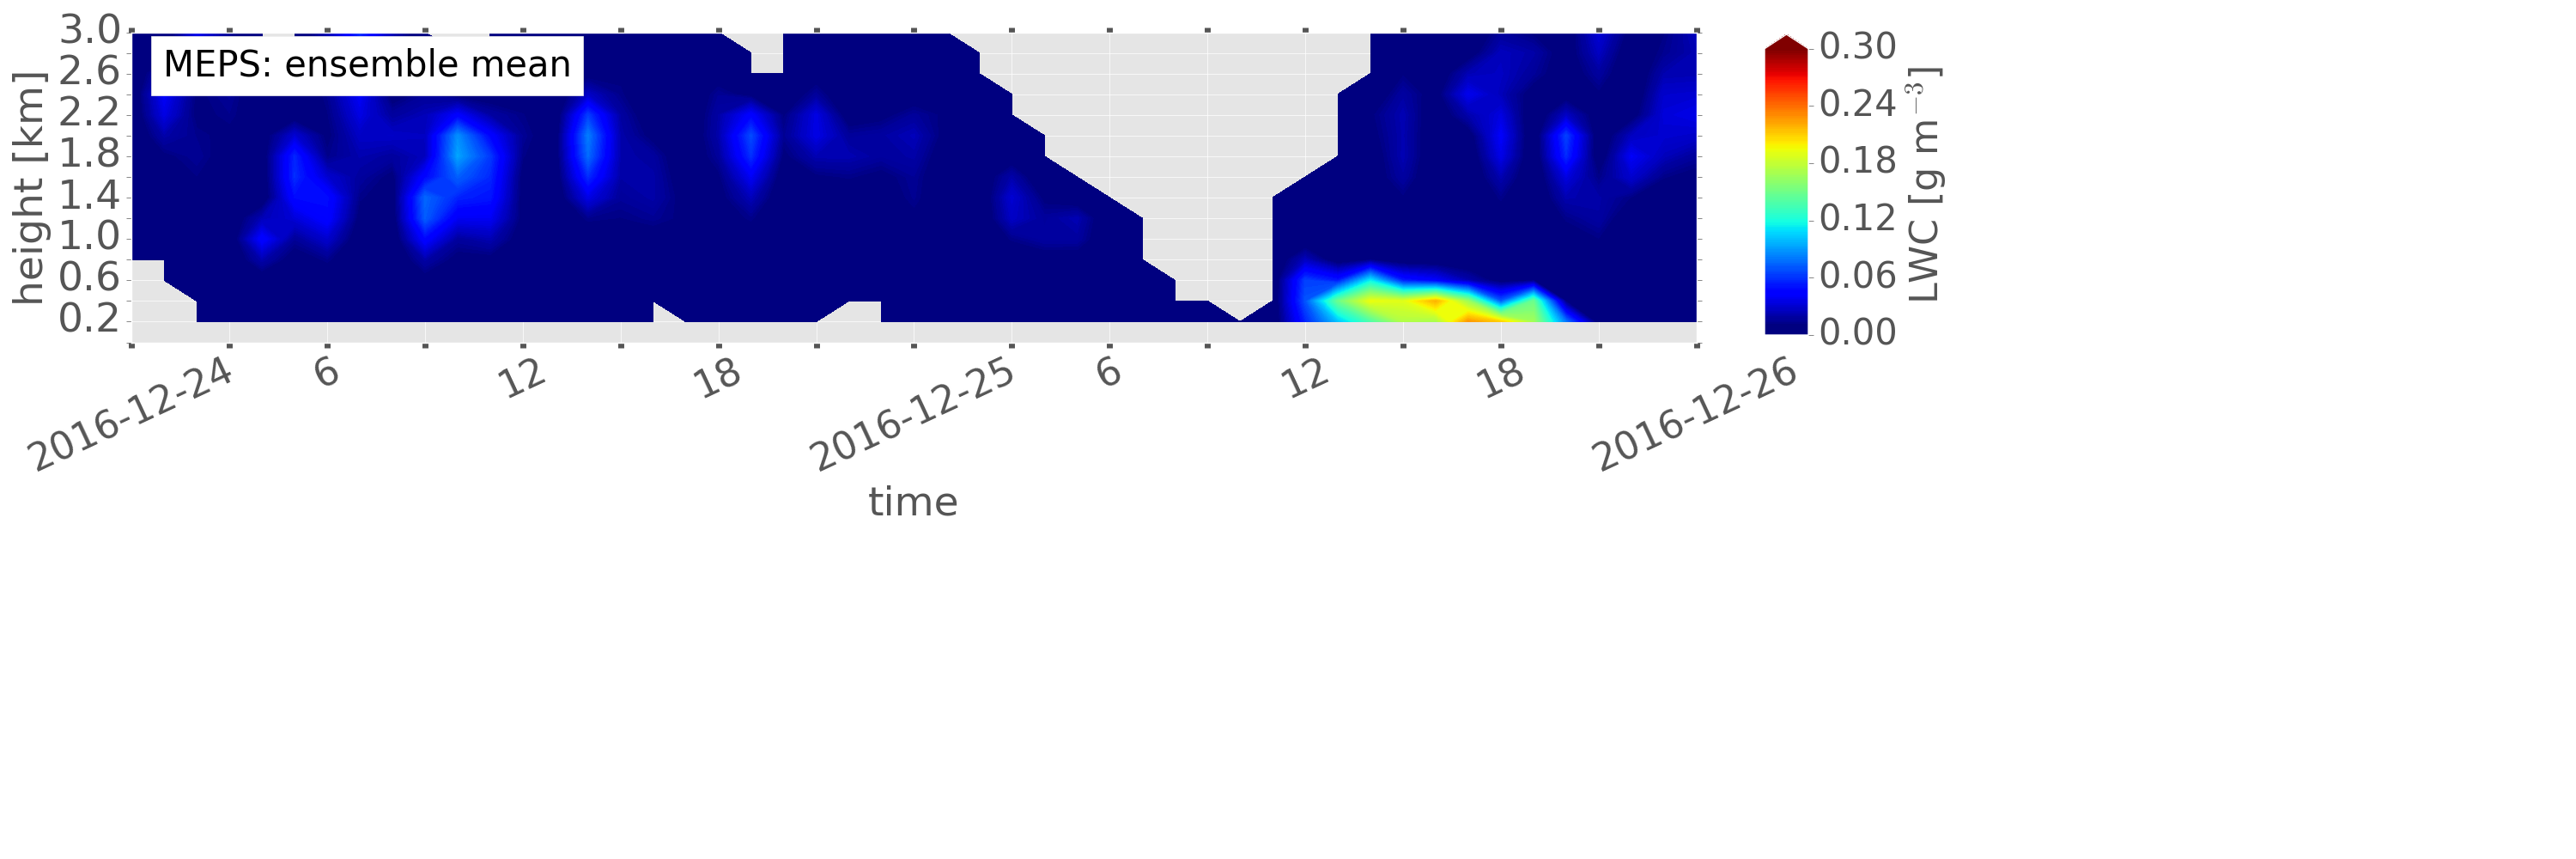
\includegraphics[trim={0.cm 11.5cm 18.5cm 0.4cm},clip,width=\textwidth]{./fig_vert_LWC_EM/20161224}
		\caption{}\label{fig:LWC:24}
	\end{subfigure}
	\begin{subfigure}[b]{\textwidth}
		\centering
		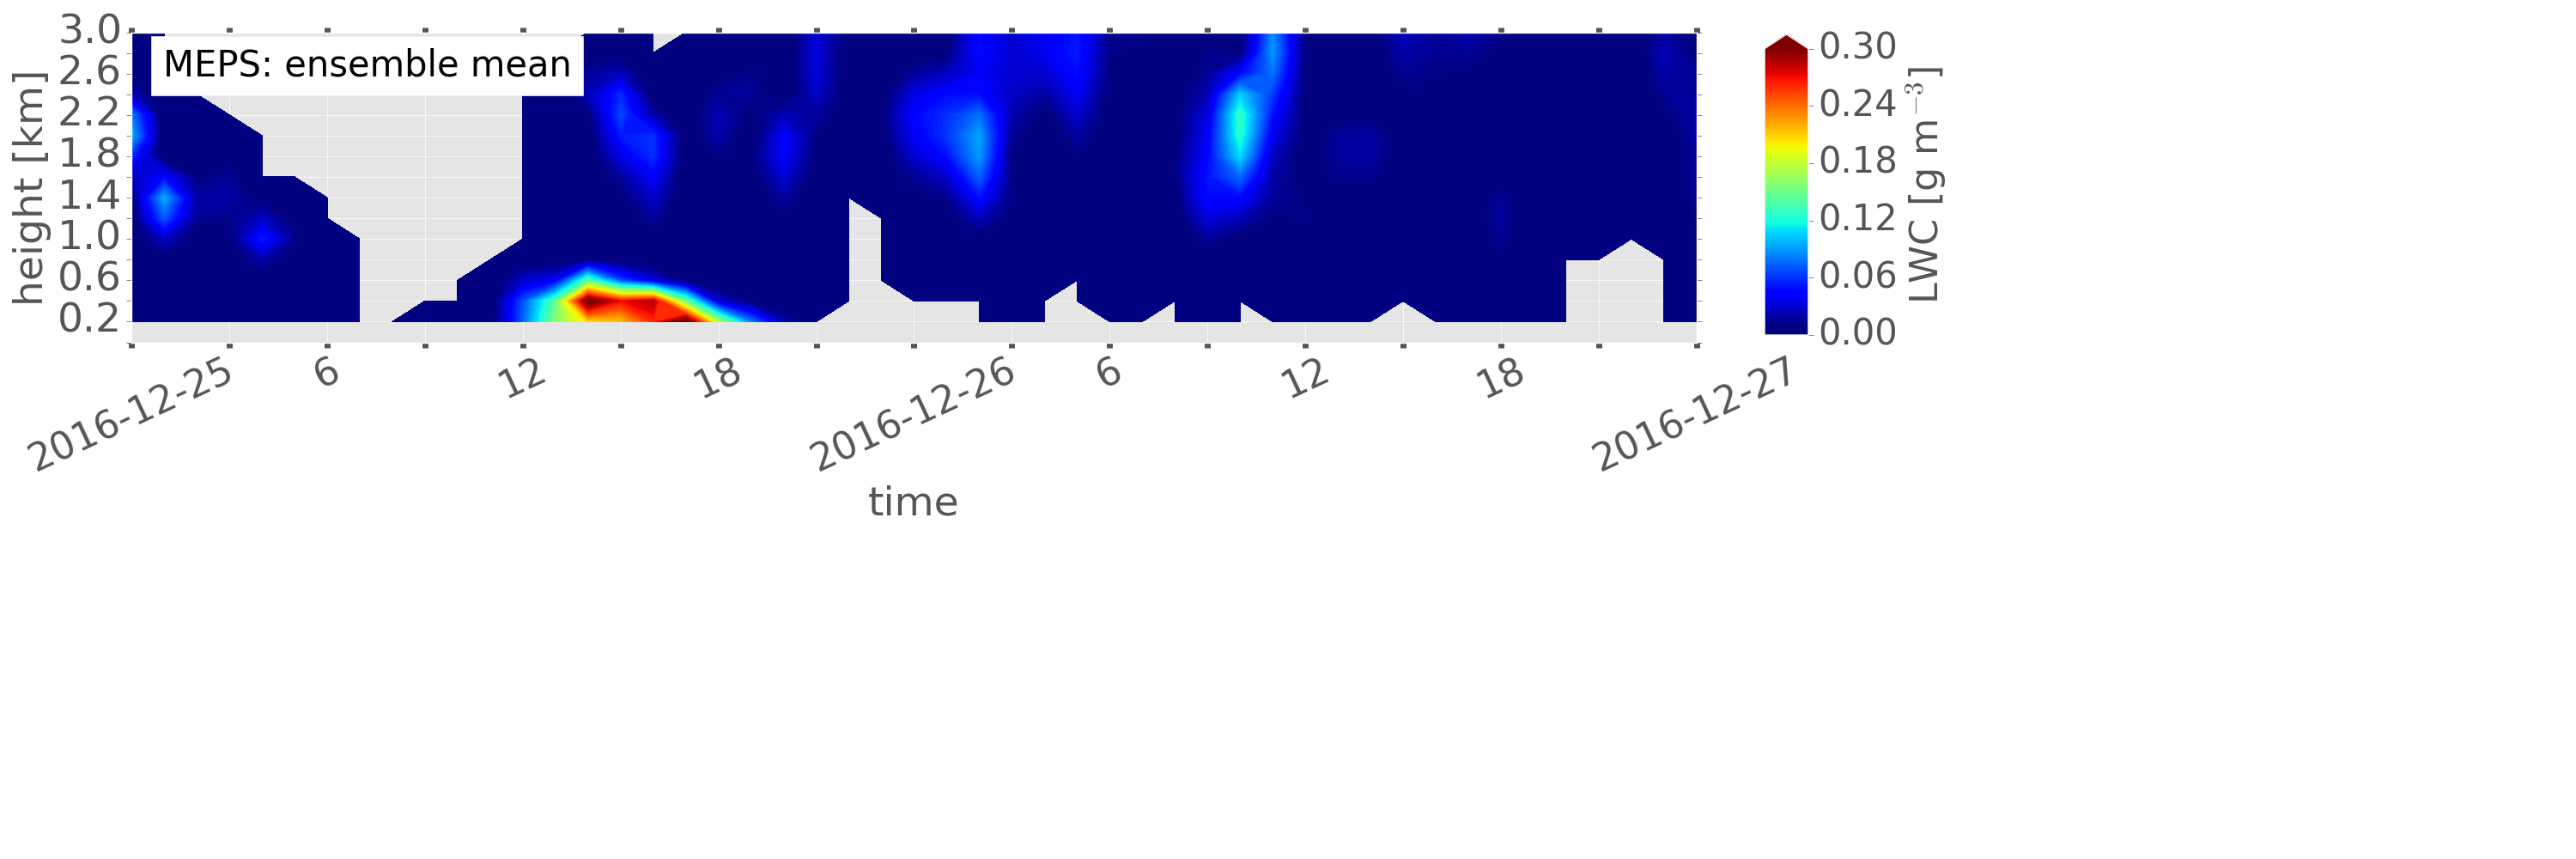
\includegraphics[trim={0.cm 10cm 18.5cm 0.4cm},clip,width=\textwidth]{./fig_vert_LWC_EM/20161225}
		\caption{}\label{fig:LWC:25}
	\end{subfigure}
	\caption{200m hourly averaged LWC forecast from MEPS with all ensemble members, neglecting missing values.
		Initialised on \SIlist{24;25}{\dec} at \SI{0}{\UTC}. Liquid water content according to the colorbar.}\label{fig:LWC:2425}
\end{figure}
%%%%%%%%%%%%%%%%%%%%%%%%%%%%%%%%%%%%%%%%%%%%%%
The \SI{25}{\dec} showed patterns of liquid precipitation (\Cref{fig:res:obs_masc}) with warm temperatures (\Cref{fig:res:sfc_temp25}) and high reflectivity (\Cref{fig:ret:refl25}) between \SIrange{12}{21}{\UTC}. High reflectivity values in \Cref{fig:ret:refl25} are present around \SI{18}{\UTC} with layer thickness up to \SI{1.2}{\km}. 
To see if liquid precipitation was predicted, the atmospheric cloud condensed water content and rainfall amount in model levels is summed. \Cref{fig:LWC:24} and \subref{fig:LWC:25} show liquid water content for initialisations at either \SI{24}{\dec} or \SI{25}{\dec}. 
Positive surface temperatures were forecasted between \SIrange{12}{21}{\UTC} (\Cref{fig:res:sfc_temp25}). Initialisations more than \SI{24}{\hour} prior show already the occurrence of the liquid layer. \Cref{fig:LWC:24} or \subref{fig:LWC:25} show also a narrow thickness up to \SI{800}{\metre}. 
In Norwegian mountainous terrain is this an important feature since precipitation change can lead to a high risk for people. The avalanche danger increases with the precipitation change especially during high wind speeds. Since MEPS forecasts the liquid layer correctly in depth and length it seems to be a good interaction between the surface model and the vertical prediction. 
This follows a high accuracy of the forecasting system and the advantage of using a high resolution convective scheme model.
\\
\\
%%% table verification %%%%%%%%%%%%%%%%%%%%%%%%%%%%%%%%%%%%%
\begin{table}[t!]
	\begin{center}
		\caption{Interpretation of the coefficient of variation for SWC.} \label{tab:verification}
		\begin{tabular}{lc|c}
			\hline\hline
			\multicolumn{2}{c|}{\textbf{Size of CV}} & {\textbf{Interpretation}} \\ 
			\multicolumn{2}{c|}{[\SI{}{\percent}]} & variability \\ \hline \hline 
			\multicolumn{2}{c|}{\numrange{0}{< 25}} & negligible  \\ \hline
			\multicolumn{2}{c|}{\numrange{25}{< 50}} & low \\ \hline
			\multicolumn{2}{c|}{\numrange{50}{< 75}} & moderate \\ \hline
			\multicolumn{2}{c|}{\numrange{75}{< 100}} & high \\ \hline
			\multicolumn{2}{c|}{\num{100} to $\infty$} & very high  \\ \hline \hline
		\end{tabular}
	\end{center}
\end{table}
%%%%%%%%%%%%%%%%%%%%%%%%%%%%%%%%%%%%%%%%%%%%%%%%%%%%%%%%%%%%%%%%%%%%%%%%%
\noindent
%A validation of how well the forecast performed is difficult to do at this state, since the time resolution of MEPS is coarse compared to the observations. 
For the first glance operates the forecast well when compared to vertical observations. One possibility is to assess the variability of all ensemble member with the coefficient of variation described in \Cref{sec:ens_mean_spread}. 
\Cref{fig:vari:EM22,fig:vari:EM25,fig:vari:EM26} show the coefficient of variation for SWC, which is the standard deviation of the ten ensemble members divided by the mean of all ensemble members. This coefficient gives the possibility to compare the SWC results for different days with different values. It follows for even a low ensemble spread of SWC (standard deviation of all ensemble members) then the different members do not need to be less variable.
\\
The grey line in \Cref{fig:ens_vari} shows the ensemble mean of the hourly predicted SWC values. The darker the colour in \Cref{fig:ens_vari} the smaller is the variation of the SWC relative to the mean. Initialisations on \SI{23}{\dec} does not exist, because it had too few ensemble members (only six) to create a reasonable verification. Therefore, the initialsation on \SI{22}{\dec} is used. The interpretation of the coefficient of variation for SWC is presented in \Cref{tab:verification}.
%%%%%%% image variability %%%%%%%%%%%%%%%%
\begin{figure}[t!]
	\centering
	\begin{subfigure}[b]{\textwidth}
		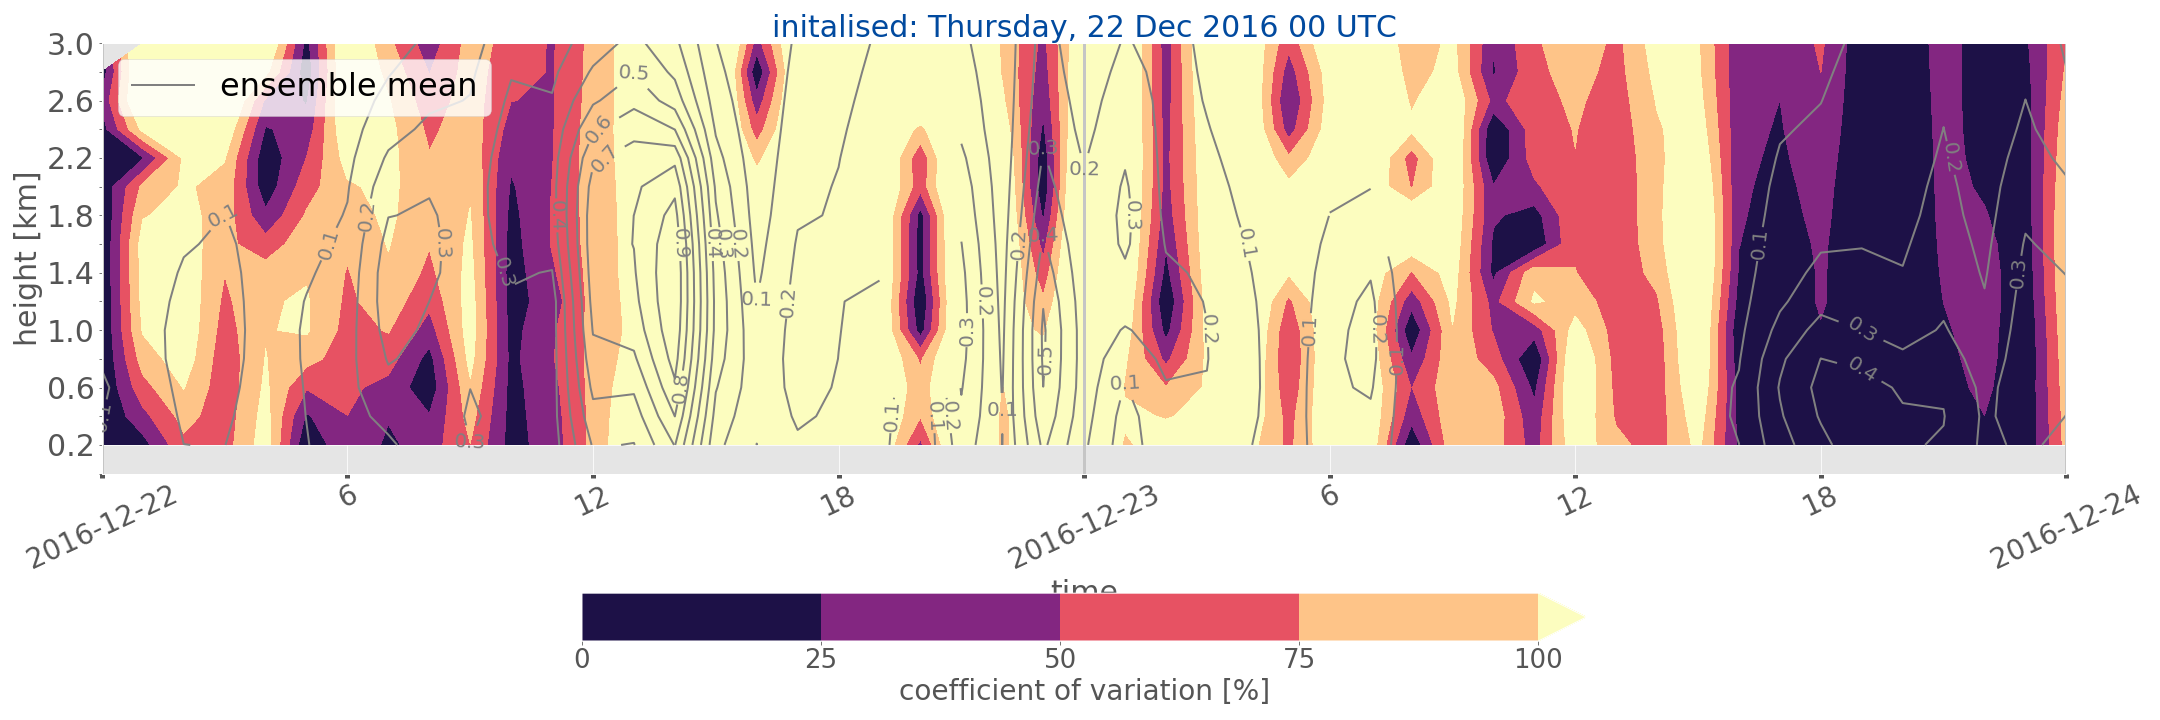
\includegraphics[trim={0cm 5cm 0cm 0cm},clip,width=\textwidth]{./fig_variation/20161222}
		\caption{}\label{fig:vari:EM22}
	\end{subfigure}
	\begin{subfigure}[b]{\textwidth}
		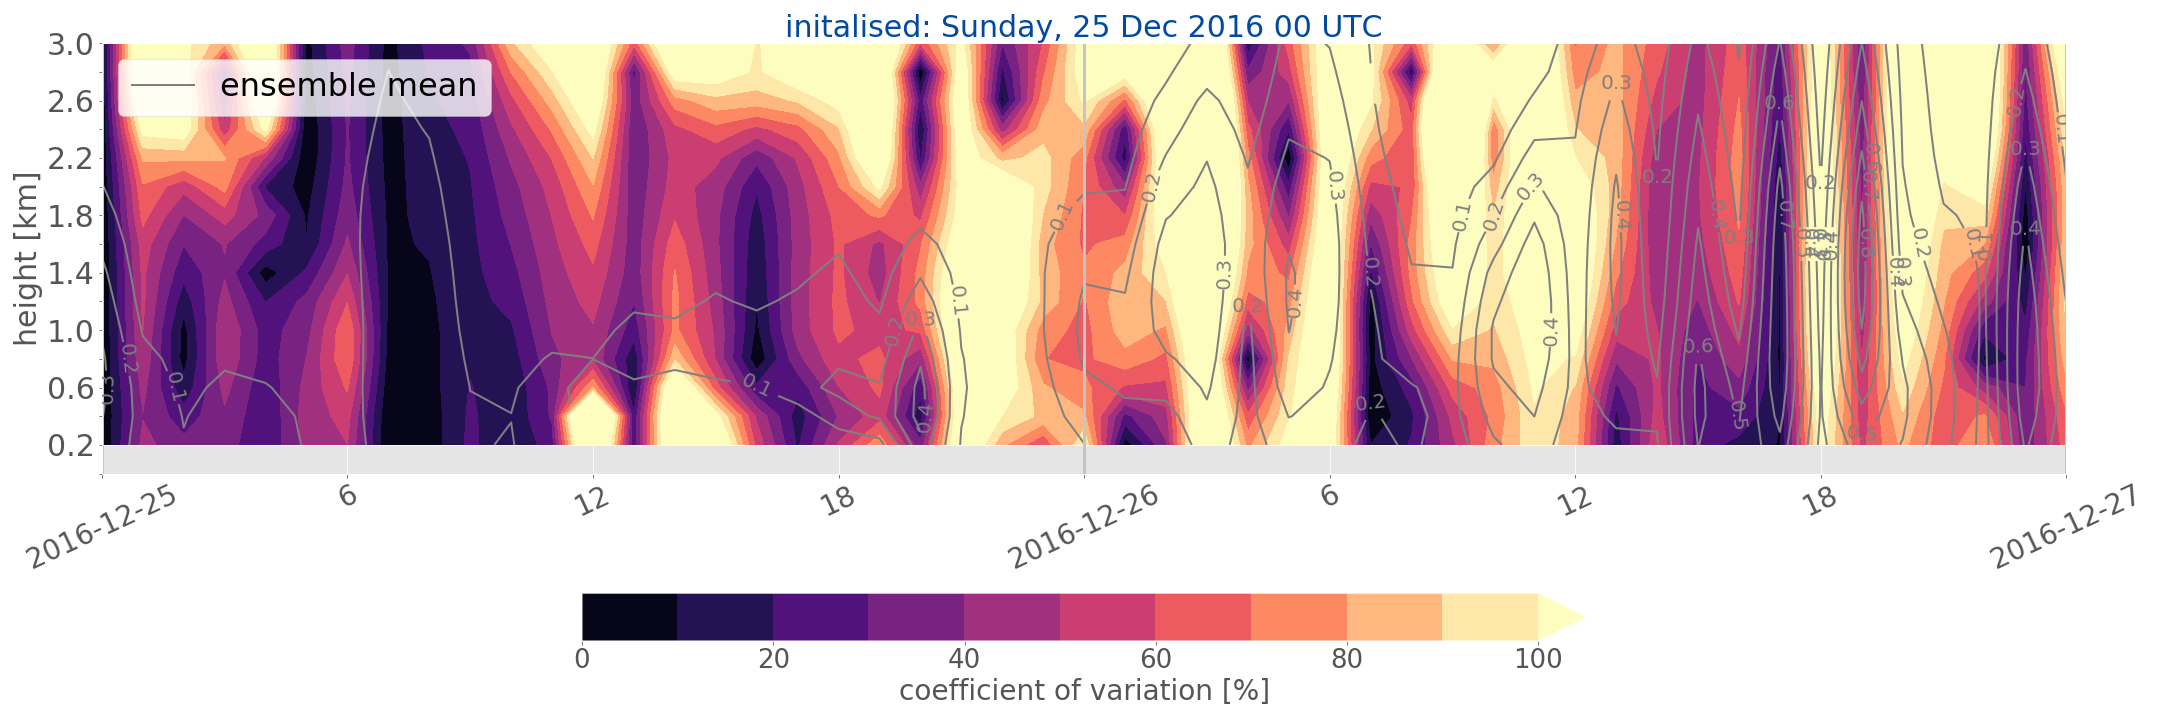
\includegraphics[trim={0cm 5cm 0cm 0cm},clip,width=\textwidth]{./fig_variation/20161225}
		\caption{}\label{fig:vari:EM25}
	\end{subfigure}
	\begin{subfigure}[b]{\textwidth}
		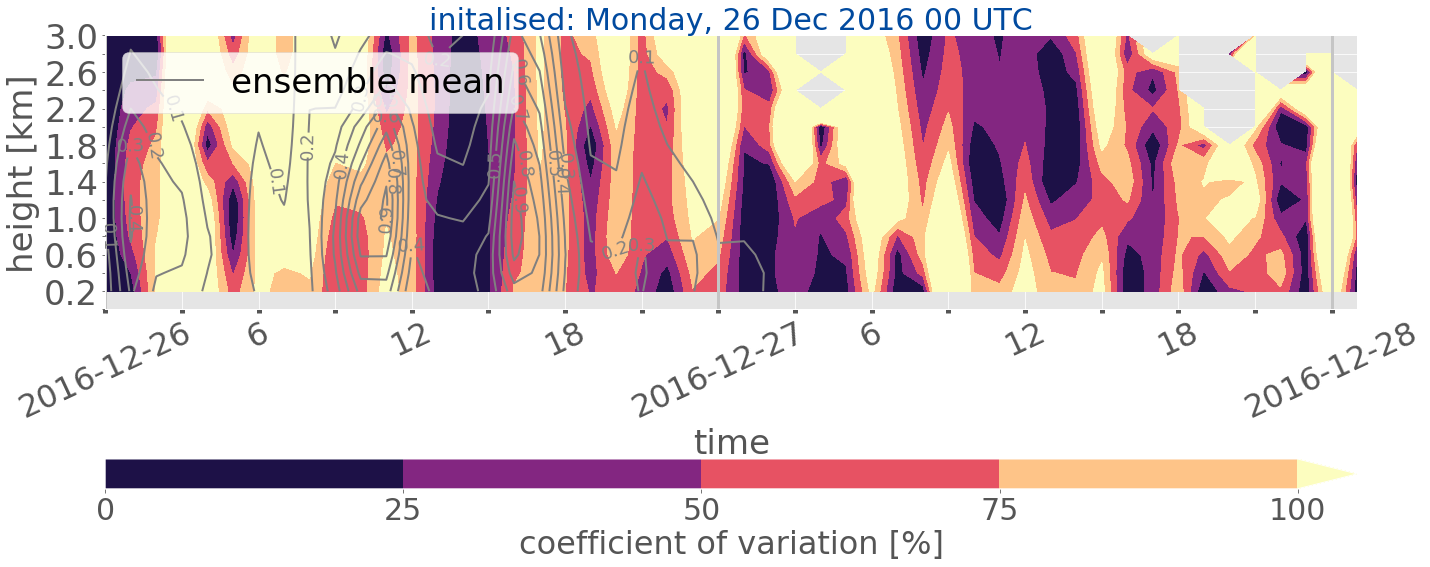
\includegraphics[trim={0cm 0cm 0cm 0cm},clip,width=\textwidth]{./fig_variation/20161226}
		\caption{}\label{fig:vari:EM26}
	\end{subfigure}
	\caption{SWC variation of the ten ensemble members of MEPS. The lighter the colour according to the colourbar the higher the variation between the perturbed ensemble members. In grey the ensemble mean of all ten members.}\label{fig:ens_vari}
\end{figure}
%%%%%%%%%%%%%%%%%%%%%%%%%%%%%%%%%%%%%%%%%%%%%%
\noindent
The CV agrees well with the prediction of the occlusion on \SI{23}{\dec} after \SI{15}{\UTC}. The variability between the members is small and show a good agreement on the occurrence of snow precipitation. \Cref{fig:EM09_22,fig:EM0923} show the same variability, where all ensemble member agree on the passage after \SI{16}{\UTC}. While comparing only six ensemble members in \Cref{fig:EM09_23}, one could assume that the uncertainty of all ensemble members during the up-slope storm is low, but not as certain as for an initialisation on \SI{22}{\dec} at \SI{0}{\UTC}.
\\
A larger difference between the ensemble members is shown for the passage of the occlusion on \SI{26}{\dec}. Initialisations on \SI{25}{\dec} present a lower variability for the passage after \SI{15}{\UTC} on \SI{26}{\dec} than initialisations less than \SI{24}{\hour} prior. Therefore, an increase of variability after shorter time and an increase in uncertainty. Again, this is not a fair comparison since hourly instantaneous values are used and there might be a time delay of half an hour about the passage which would follow it is not seen in the model forecast. 
\\
Another way to see how the MEPS forecast performed compared to the vertical observations can be done by correlating the observed SWP with the ensemble member snow water content.
% %%% fig correlation %%%%%%%%%%%%%%%%%%%%%%%%%%%%%%%%%%%%%
% \begin{figure}[t!]
% 	\centering
%     \begin{subfigure}[b]{0.49\textwidth}
%     	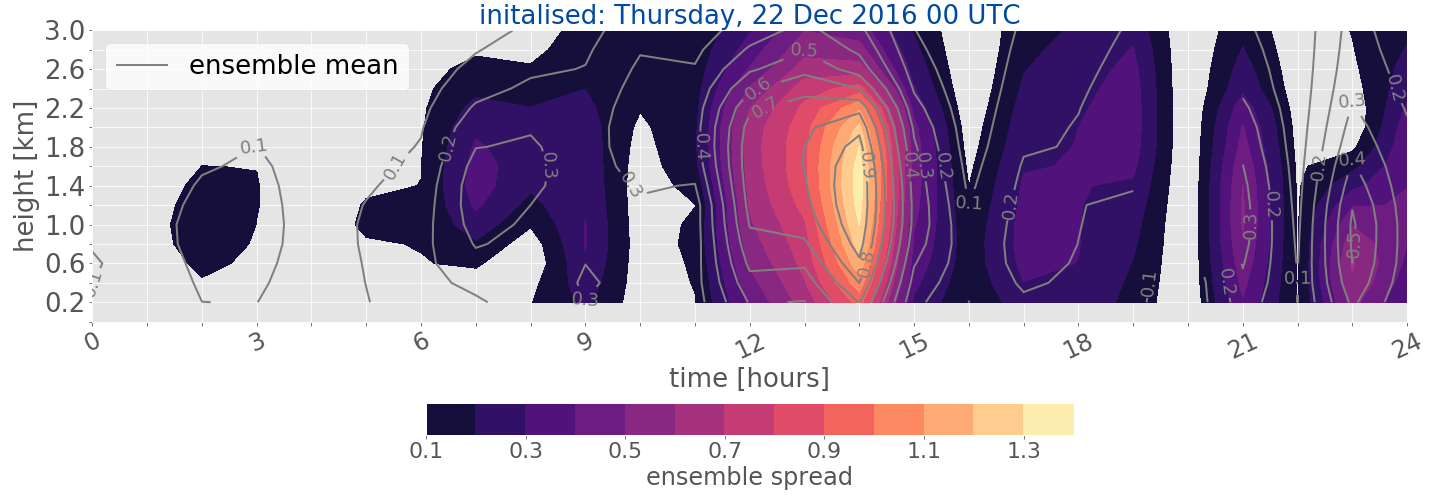
\includegraphics[width=\textwidth]{./fig_SWP_scat/20161222}
%         \caption{}\label{fig:scatSWP:22}
%     \end{subfigure}
%     \begin{subfigure}[b]{0.49\textwidth}
%     	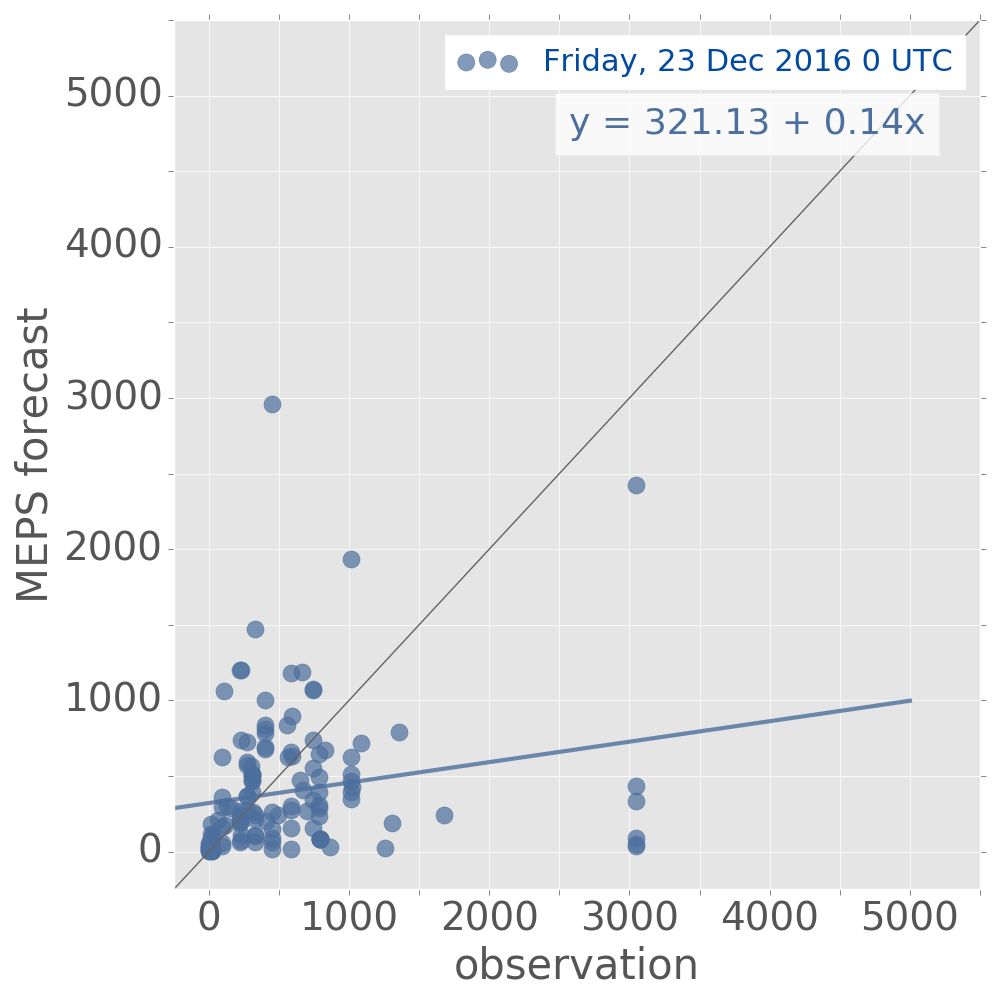
\includegraphics[width=\textwidth]{./fig_SWP_scat/20161223}
%         \caption{}\label{fig:scatSWP:23}
%     \end{subfigure}
%     \begin{subfigure}[b]{0.49\textwidth}
%     	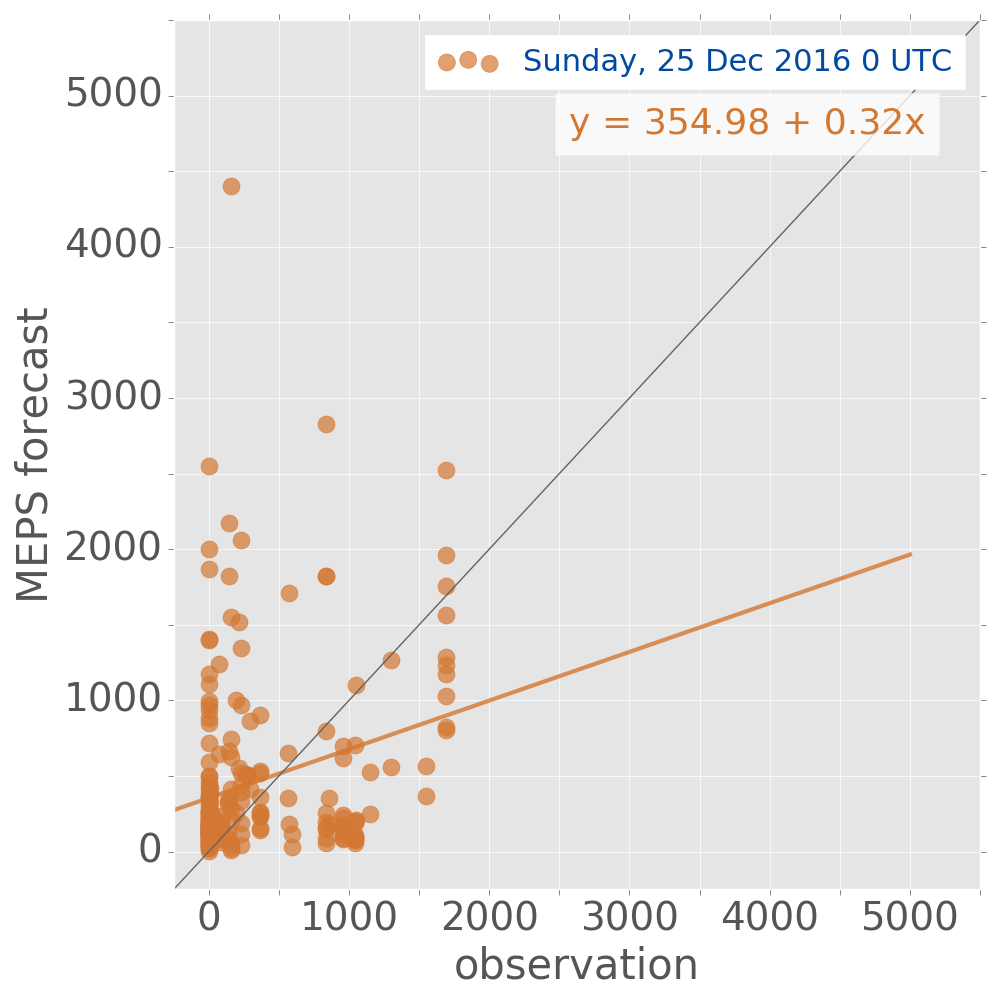
\includegraphics[width=\textwidth]{./fig_SWP_scat/20161225}
%         \caption{}\label{fig:scatSWP:25}
%     \end{subfigure}
%     \begin{subfigure}[b]{0.49\textwidth}
%     	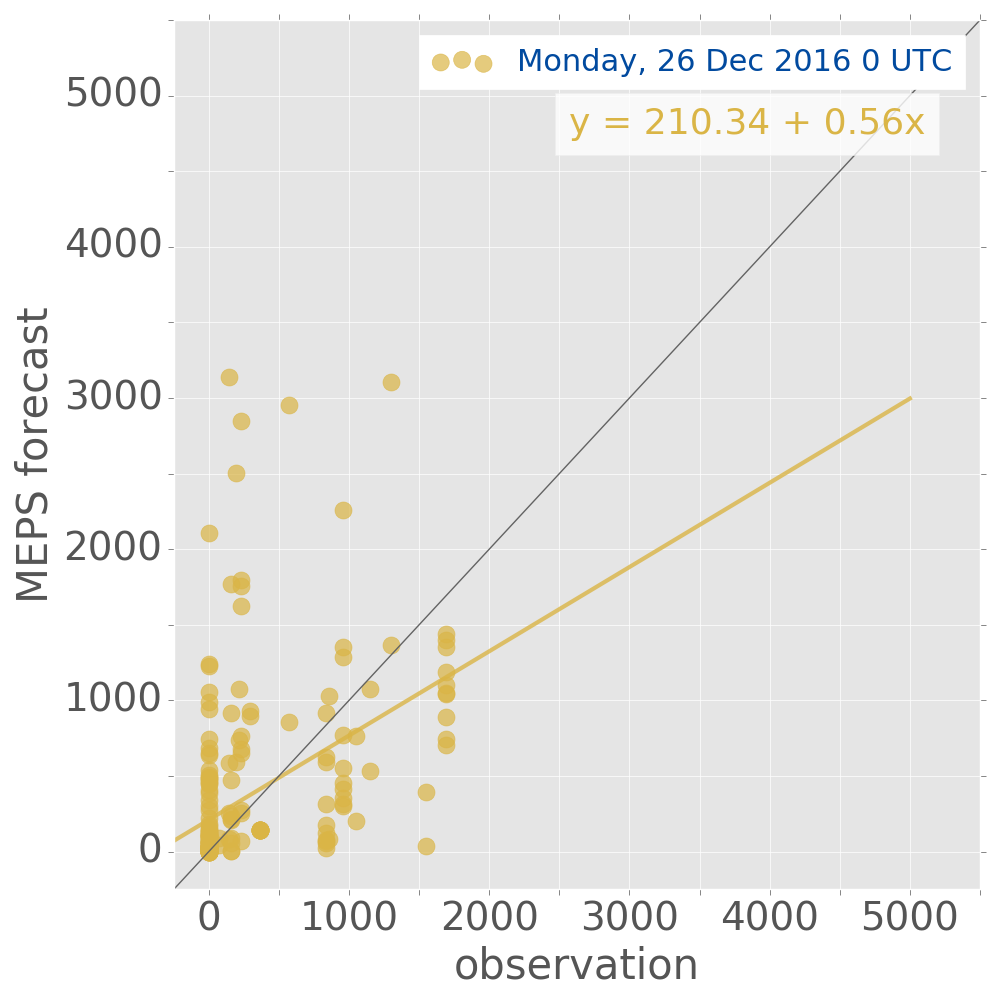
\includegraphics[width=\textwidth]{./fig_SWP_scat/20161226}
%         \caption{}\label{fig:scatSWP:26}
%     \end{subfigure}
%     \caption{}\label{fig:scatSWP}
% \end{figure}
% %%%%%%%%%%%%%%%%%%%%%%%%%%%%%%%%%%%%%%%%%%%%%%%%%%%%%%%%%%%%%%%%%%%%%%%%%
\\
\\
One question to answer in this work is if the operational model MEPS gets large scale features correctly. As discussed here and in \Cref{sec:res:large_scale_sfc} it seems that the model is able to cover the development of large scale features and its associated precipitation. Even with the intensification of the storm seems MEPS to be able to predict extreme events such as the Christmas event, but might have some issues predicting fast transitions of frontal boundaries. 
\\
MEPS is also able to distinguish between liquid and solid precipitation in layer thickness and duration for time resolution of one hour. This can be a major advantage since a change in temperature and associated precipitation transformation can lead to high safety issues in the Norwegian mountains, especially during winter. With the knowledge more than \SI{24}{\hour} prior can risk notice be send out to the population and rescue teams can prepare in advance. Furthermore, roads and train tracks can be closed to increase the safety of people.
%\\
\textcolor{red}{I'm not sure if the above mentioned should be here?! }
%%%%%%%%%%%%%%%%%%%%%%%%%%%%%%%%%%%%%%%%%%%%%%%%%%%%%%%%%%%%%%%%%%%%%%%%%%
%%%%%%%%% surface overestimation - vertical? %%%%%%%%%%%%%%
%\section{Surface overestimation and the vertical}

%%%%%%%%% Local affects %%%%%%%%%%%%%%
\section{Orographic influence on precipitation}\label{sec:res:oro_infl}
The Haukeliseter is suspended to high wind speeds during the winter. The previous results have shown, that wind plays an important role on the precipitation. The mountain plateau is surrounded by higher mountains to the west and more open to the south east \citep{wolff_measurements_2013,wolff_derivation_2015}, this orography seems to influence the vertical precipitation pattern. The correlation between wind speed observations and forecast have shown an overestimation of predicted wind speed throughout the event (\Cref{fig:scat:ws2123} and \subref{fig:scat:ws2426}). \citet{muller_arome-metcoop:_2017} already mentioned the weakness of too strong wind prediction in AROME-MetCoOp.
\\
On \SIlist{21;23}{\dec} wind directions from the south-east and south were observed, respectively. As earlier discussed in \Cref{sec:res:large_scale_sfc} and \subref{sec:res:large_scale_vert} was the wind change associated with the occlusion passage on \SI{23}{\dec}. The wind direction on \SI{21}{\dec} change was also related to the large scale synoptic flow but was not associated with a frontal passage. A comparison with the large scale weather analysis from ECMWF shows, that the large scale surface wind is from the south-west at \SI{6}{\UTC} on \SI{21}{\dec} (\Cref{fig:GP21_06}) and has changed to west at \SI{12}{\UTC} (\Cref{fig:GP21_12}). The observations at the Haukeliseter site show between \SIrange{6}{12}{\UTC} wind from south-east, while the predicted wind direction is from south in \Cref{fig:res:sfc_wd21}. The local wind direction influenced the precipitation pattern in the vertical in the matter that a more consistent storm structure was observed and predicted between \SIrange{9}{12} {\UTC} (\Cref{fig:SWC:ret_21,fig:SWC_EM:21,fig:SWC3h:21}). 
%%%%%%%%% image SWC retrieval MEPS 21 %%%%%%%%%%%%%%
\begin{figure}[ht!]
	\centering
	% 21/12
	\begin{subfigure}[t]{\textwidth}
		\centering
		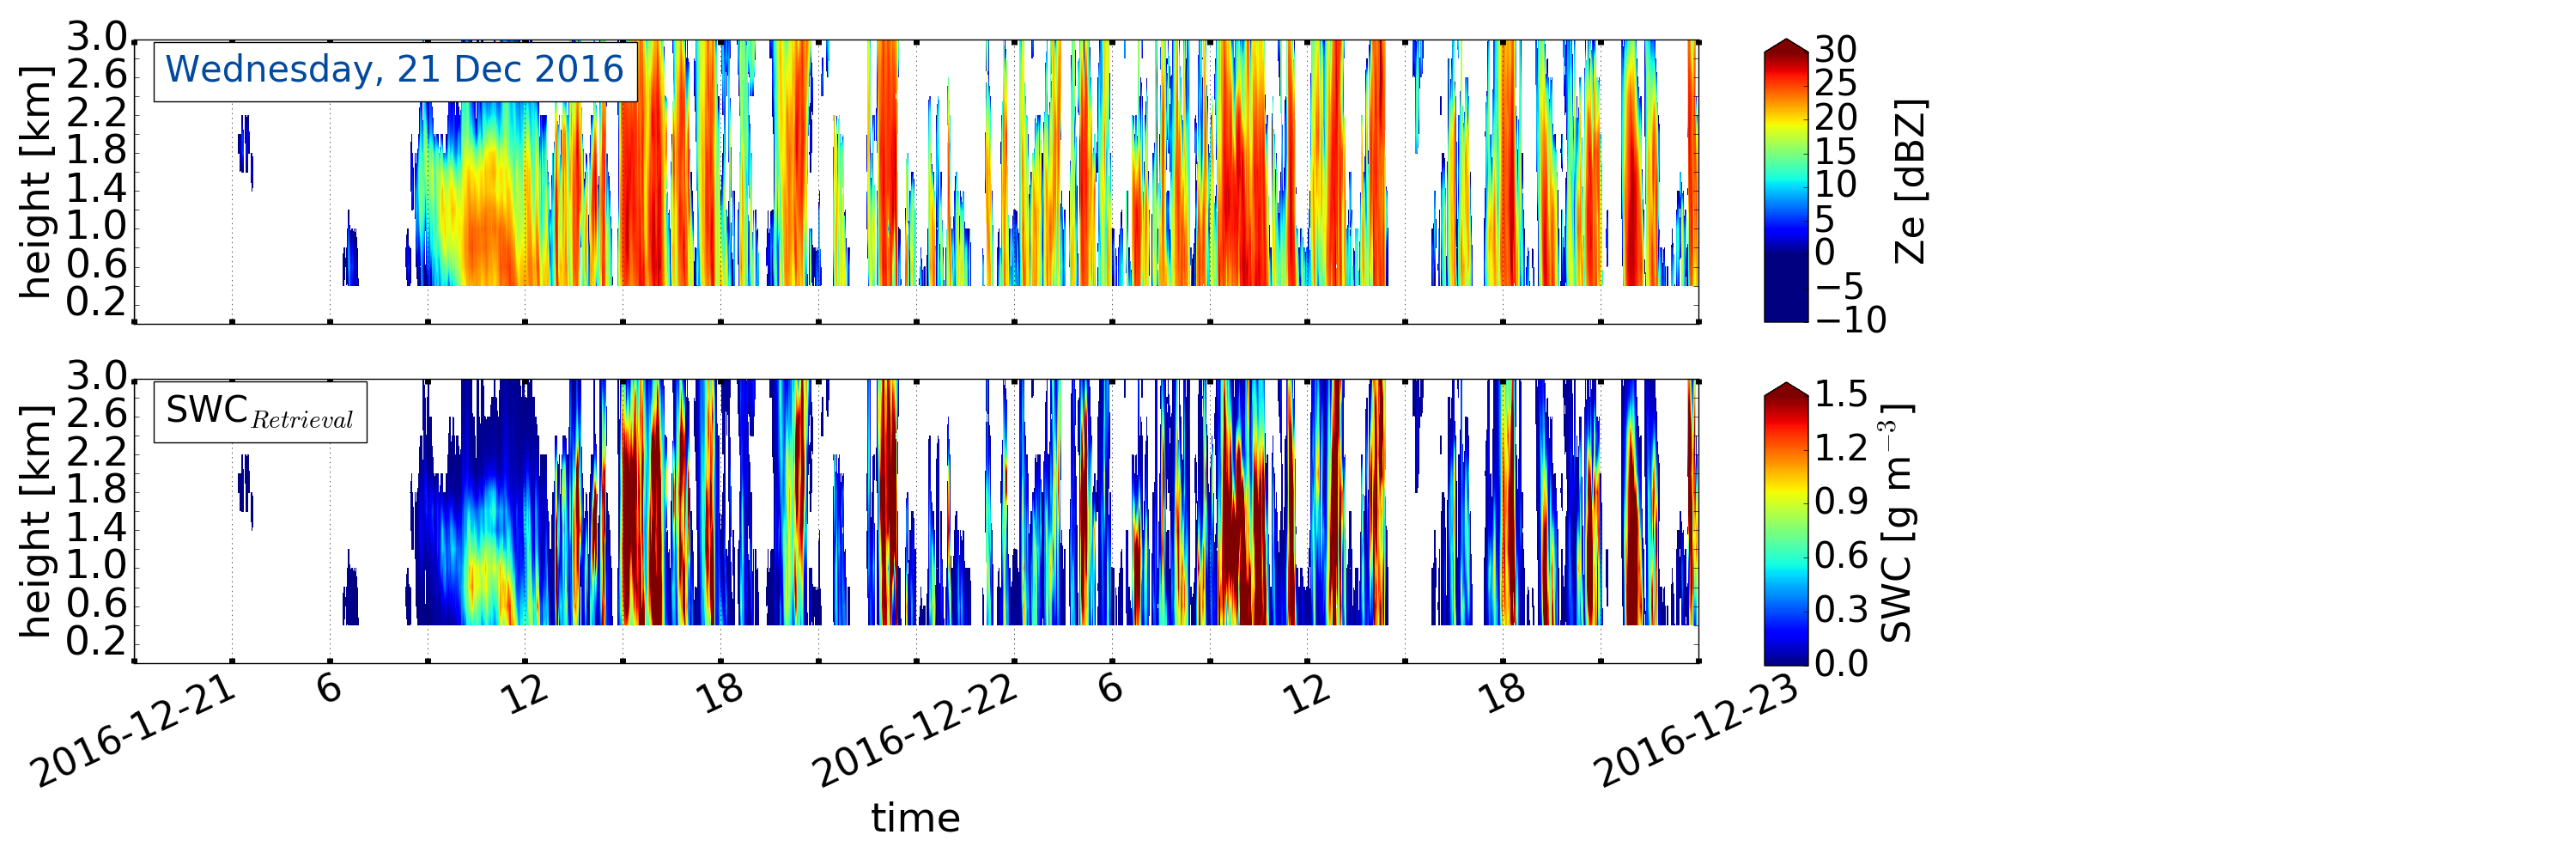
\includegraphics[trim={0.cm 2.2cm 19.cm 0.5cm},clip,width=0.9\textwidth]{./fig_obs_ret/20161221}
		\caption{}\label{fig:SWC:ret_21}
	\end{subfigure}
	% EM
	\begin{subfigure}[t]{\textwidth}
		\centering
		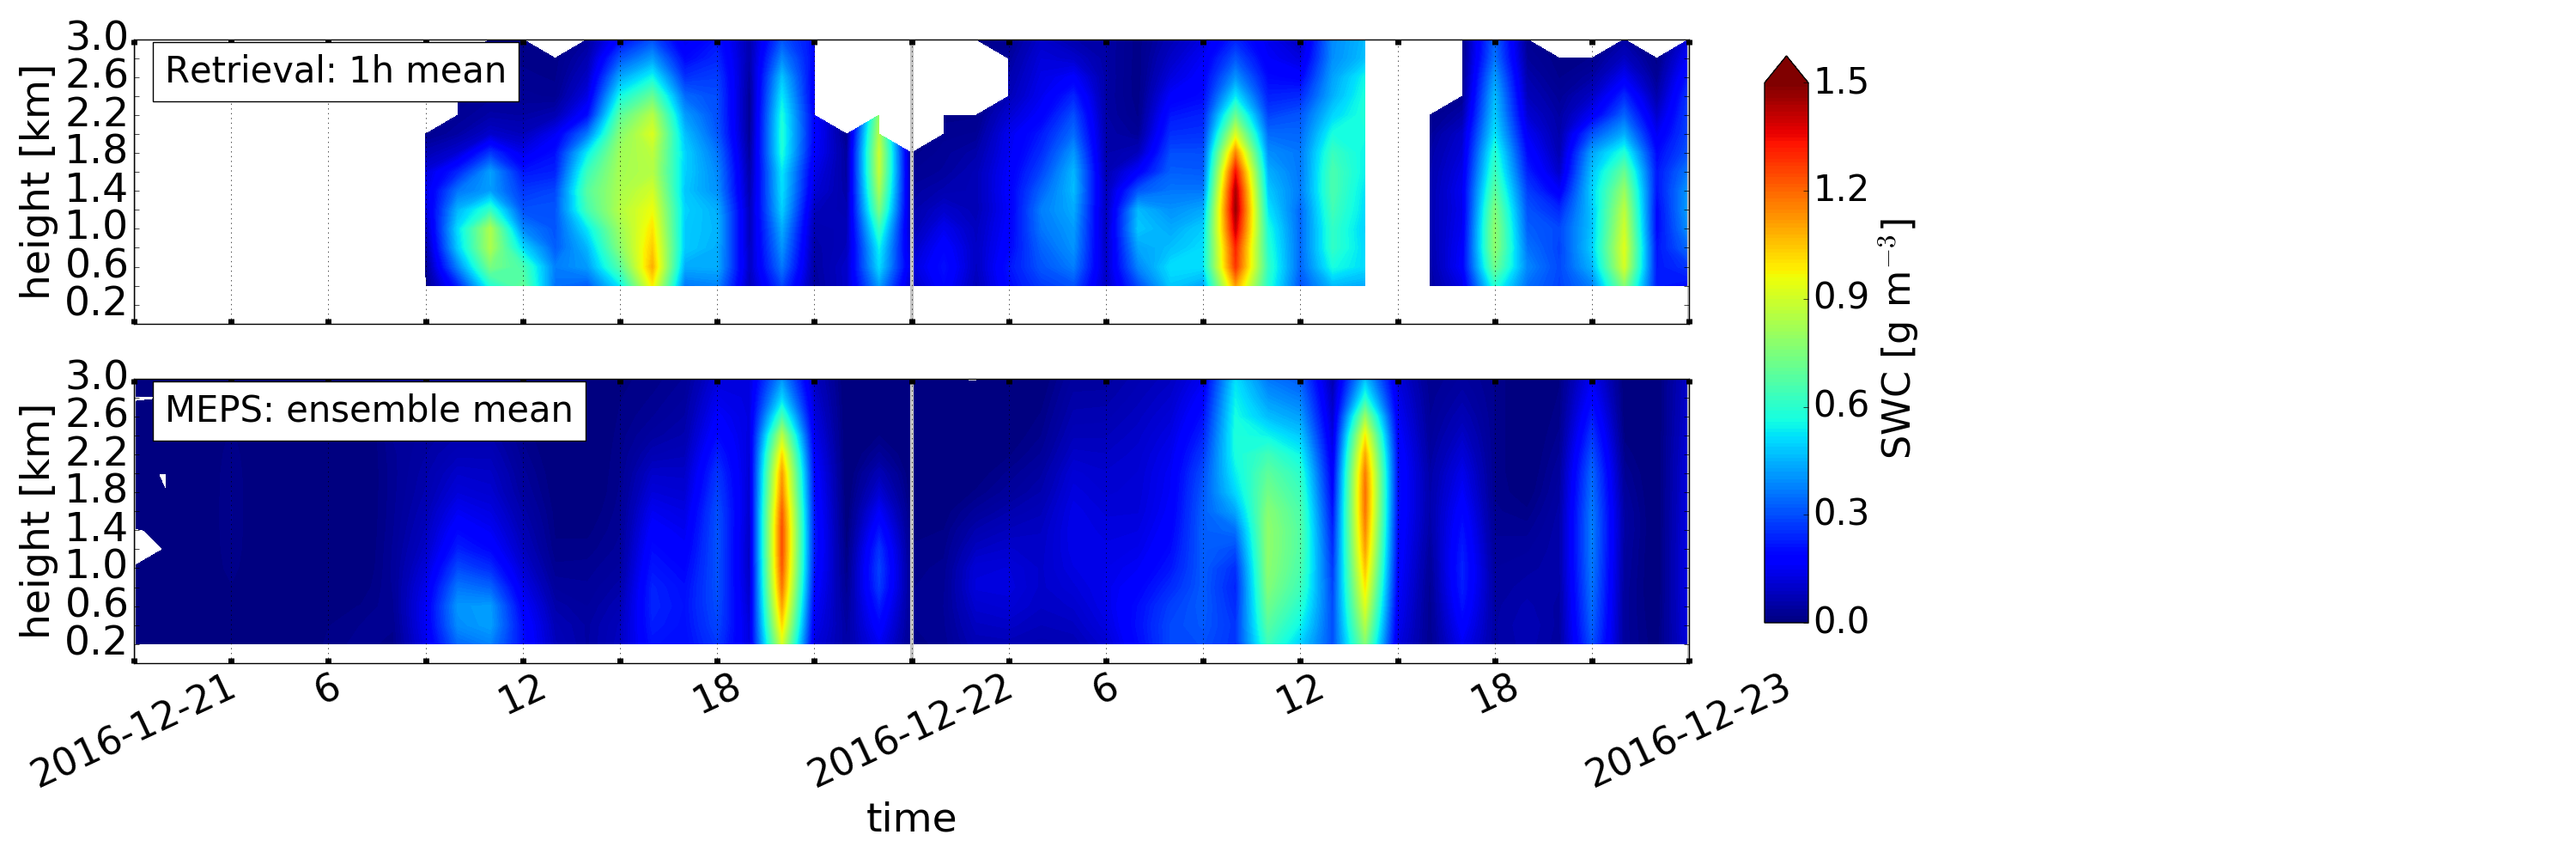
\includegraphics[trim={0.cm 2.2cm 19.cm 0.5cm},clip,width=0.9\textwidth]{./fig_vert_SWC_EM/20161221}
		\caption{}\label{fig:SWC_EM:21}
	\end{subfigure}
	% 3h
	\begin{subfigure}[t]{\textwidth}
		\centering
		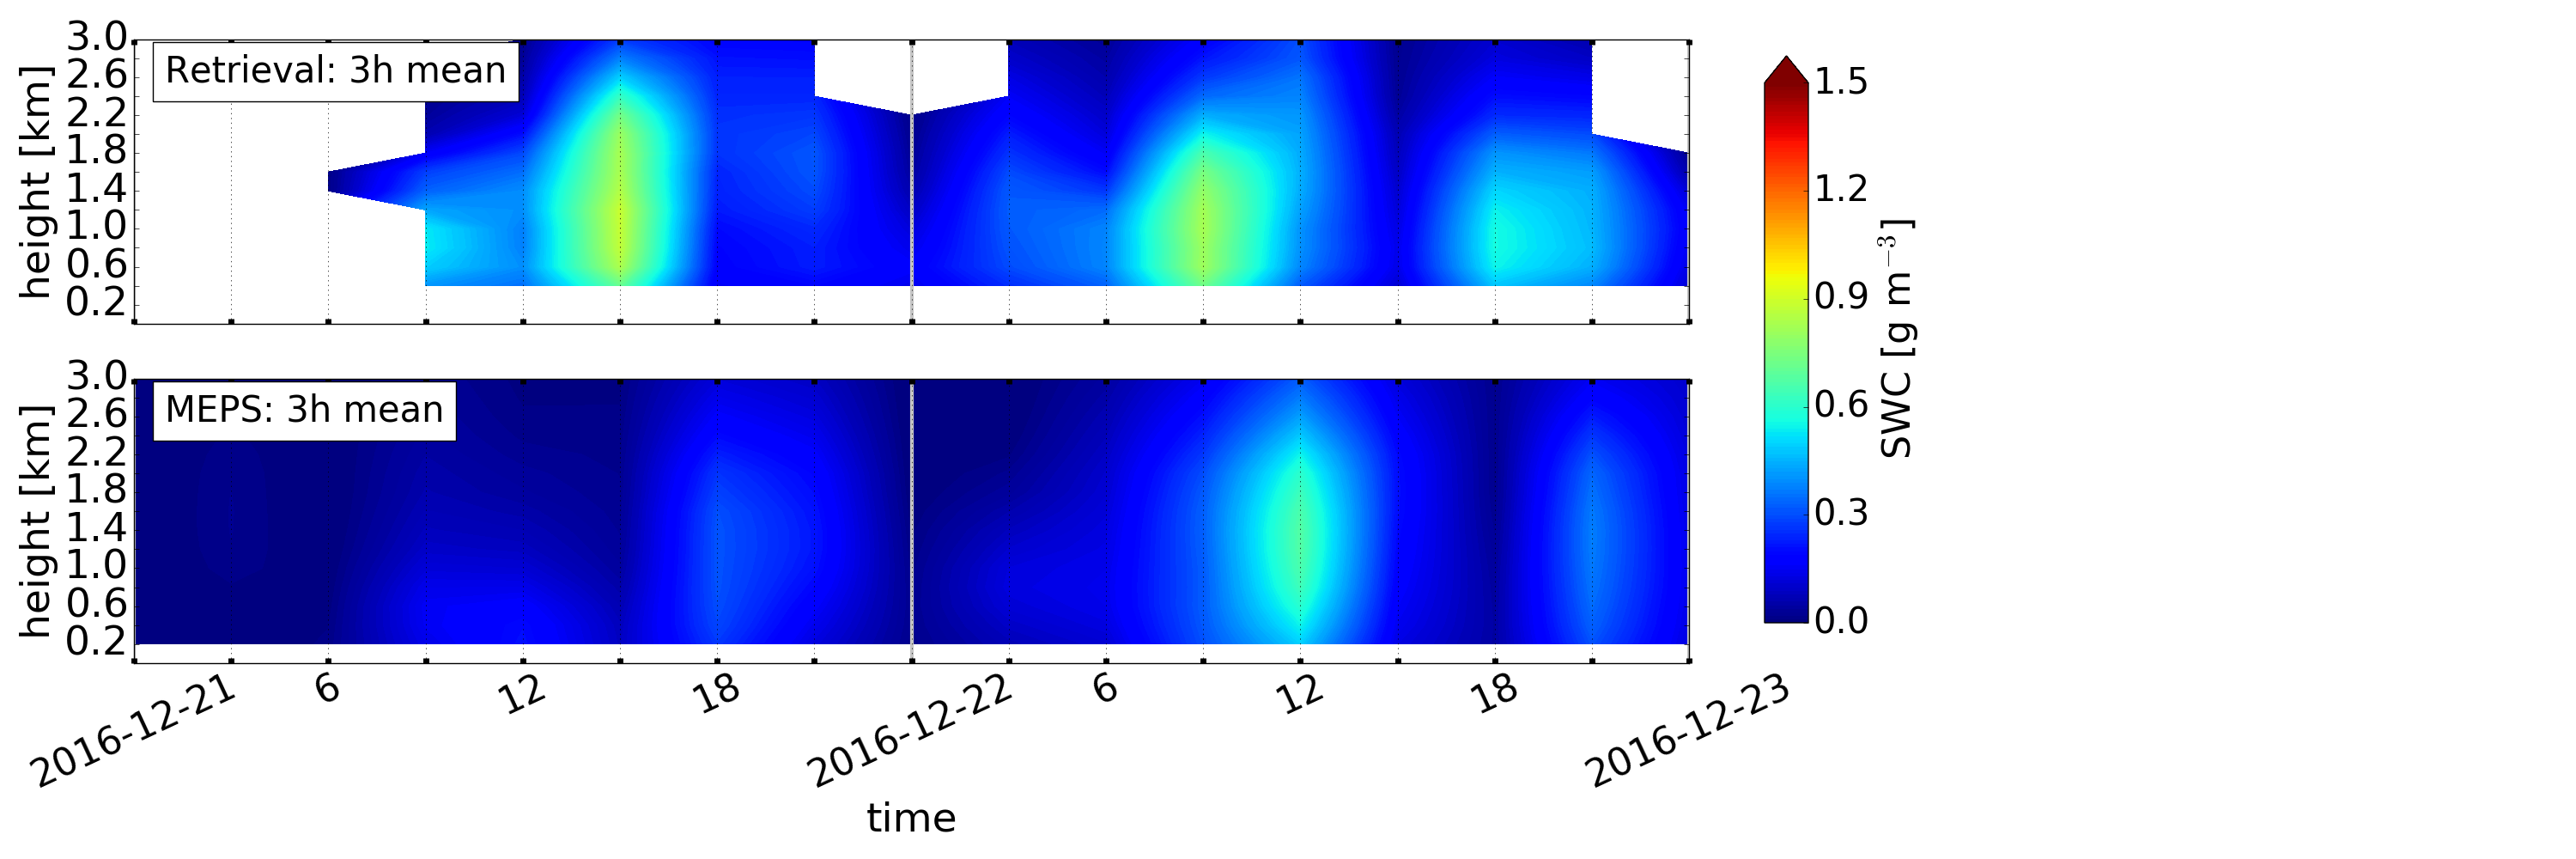
\includegraphics[trim={0.cm 0.8cm 19.cm 0.5cm},clip,width=0.9\textwidth]{./fig_vert_SWC_3h/20161221}
		\caption{}\label{fig:SWC3h:21}
	\end{subfigure}
	\caption{Initialisation \SI{21}{\dec} \SI{0}{\UTC}. 
		(\protect\subref{fig:SWC:ret_21},\protect\subref{fig:SWC:ret_24}) Upper panel: MRR reflectivity for \SI{48}{\hour}, lower panel minutely retrieved SWC. 
		(\protect\subref{fig:SWC_EM:21}, \protect\subref{fig:SWC_EM:24}) Upper panel: hourly averaged retrieved SWC, lower panel instantaneous hourly averaged forecast of all ensemble member SWC, neglecting missing values. 
		(\protect\subref{fig:SWC3h:21}, \protect\subref{fig:SWC3h:24}) Upper panel three hourly averaged retrieved SWC, lower panel instantaneous three hourly averaged forecast of all ensemble member SWC.   }\label{fig:ret:SWC21_24}
\end{figure}
%%%%%%%%%%%%%%%%%%%%%%%%%%%%%%%%%%%%%%%%%%%%%%
\noindent
Both days show a more consistent storm structure with not as intense snow water content than for storm patterns from the west. 
\Cref{fig:site:kartverket} presents the local topography around Haukeliseter and \Cref{fig:meps:site} shows the topography resolved by MEPS. It shows that MEPS is able to cover some of the complex structure around the site, with the higher mountain to the west and the valley to the south-east. The prediction model seems to forecast the wind direction overall well, only on \SI{21}{\dec} before \SI{10}{\UTC} is a south instead of a south-east wind predicted. It displays that even if the large scale wind is from the south-west is the local wind rather from the south or south-east. The orography in \Cref{fig:site:kartverket} lets assume that large scale south-west wind is forced along the valley laying in south-east direction. As \Cref{fig:SWC_EM:21} indicates is the model obviously able to cover almost the exact timing of the up-slope storm pattern. The variability of each ensemble member is again presented in \Cref{fig:EM09_21}. It shows that almost all ensemble member agree on the occurrence of the storm pattern during \SIrange{9}{12}{\UTC}.
\\
Wind from the west and therefore over mountains followed always a pulsing with more intense precipitation in the vertical (\Cref{fig:ret:SWC} and \ref{fig:ret:SWC2}). This effect might be related to wave breaking at the mountain and result into a pulsing precipitation pattern. More precipitation events need to be studied to understand this effect around the Haukeliseter site. MEPS seems not to cover all pulses during the course of a day, which is related to the time resolution of the forecast values. Since the prediction values exist only every hour the model might miss some of the high pulses \SI{30}{\minute} before or after the occurrence. 
\\
One outcome of the presented study is that MEPS is able to resolve the local topography and predicts the wind direction in almost all the cases correctly. It did not cover the south-east wind direction on \SI{21}{\dec}, which must be related to the local topography. It seems more intuitive for the model to force large scale south-westerly flow into south direction. As seen in \Cref{fig:meps:site} must the wind go along the \SI{7.2}{\degree} longitude, since a higher elevation is to the west and a \SI{1350}{\metre} high mountain to the east. This true prediction of wind direction leads then to the correct estimation of vertical precipitation patterns. 
%%%%%%%%% image SWC retrieval MEPS 24 %%%%%%%%%%%%%%
\begin{figure}[ht!]\ContinuedFloat
	\centering
	% 24/12
	\begin{subfigure}[t]{\textwidth}
		\centering
		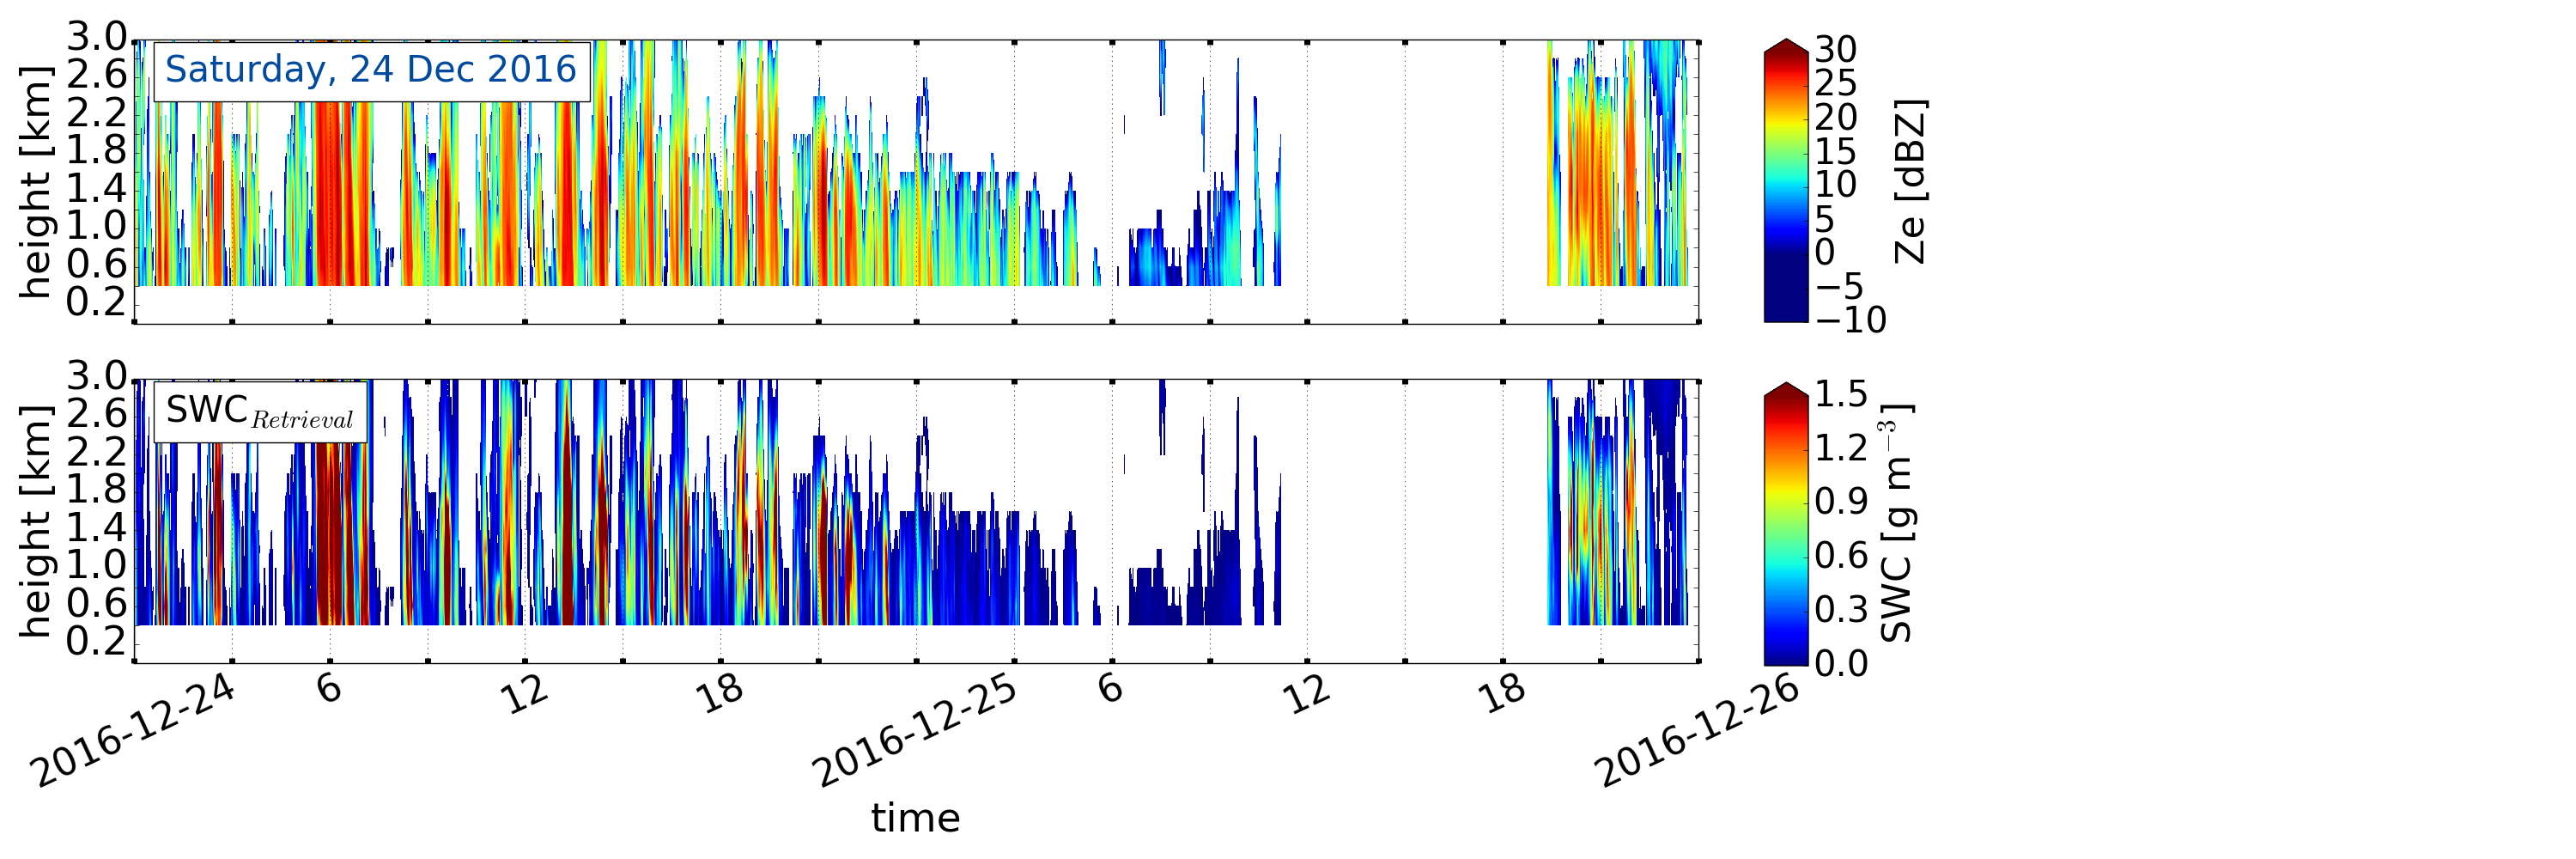
\includegraphics[trim={0.cm 2.2cm 19.cm 0.5cm},clip,width=0.9\textwidth]{./fig_obs_ret/20161224}
		\caption{}\label{fig:SWC:ret_24}
	\end{subfigure}
	% EM
	\begin{subfigure}[t]{\textwidth}
		\centering
		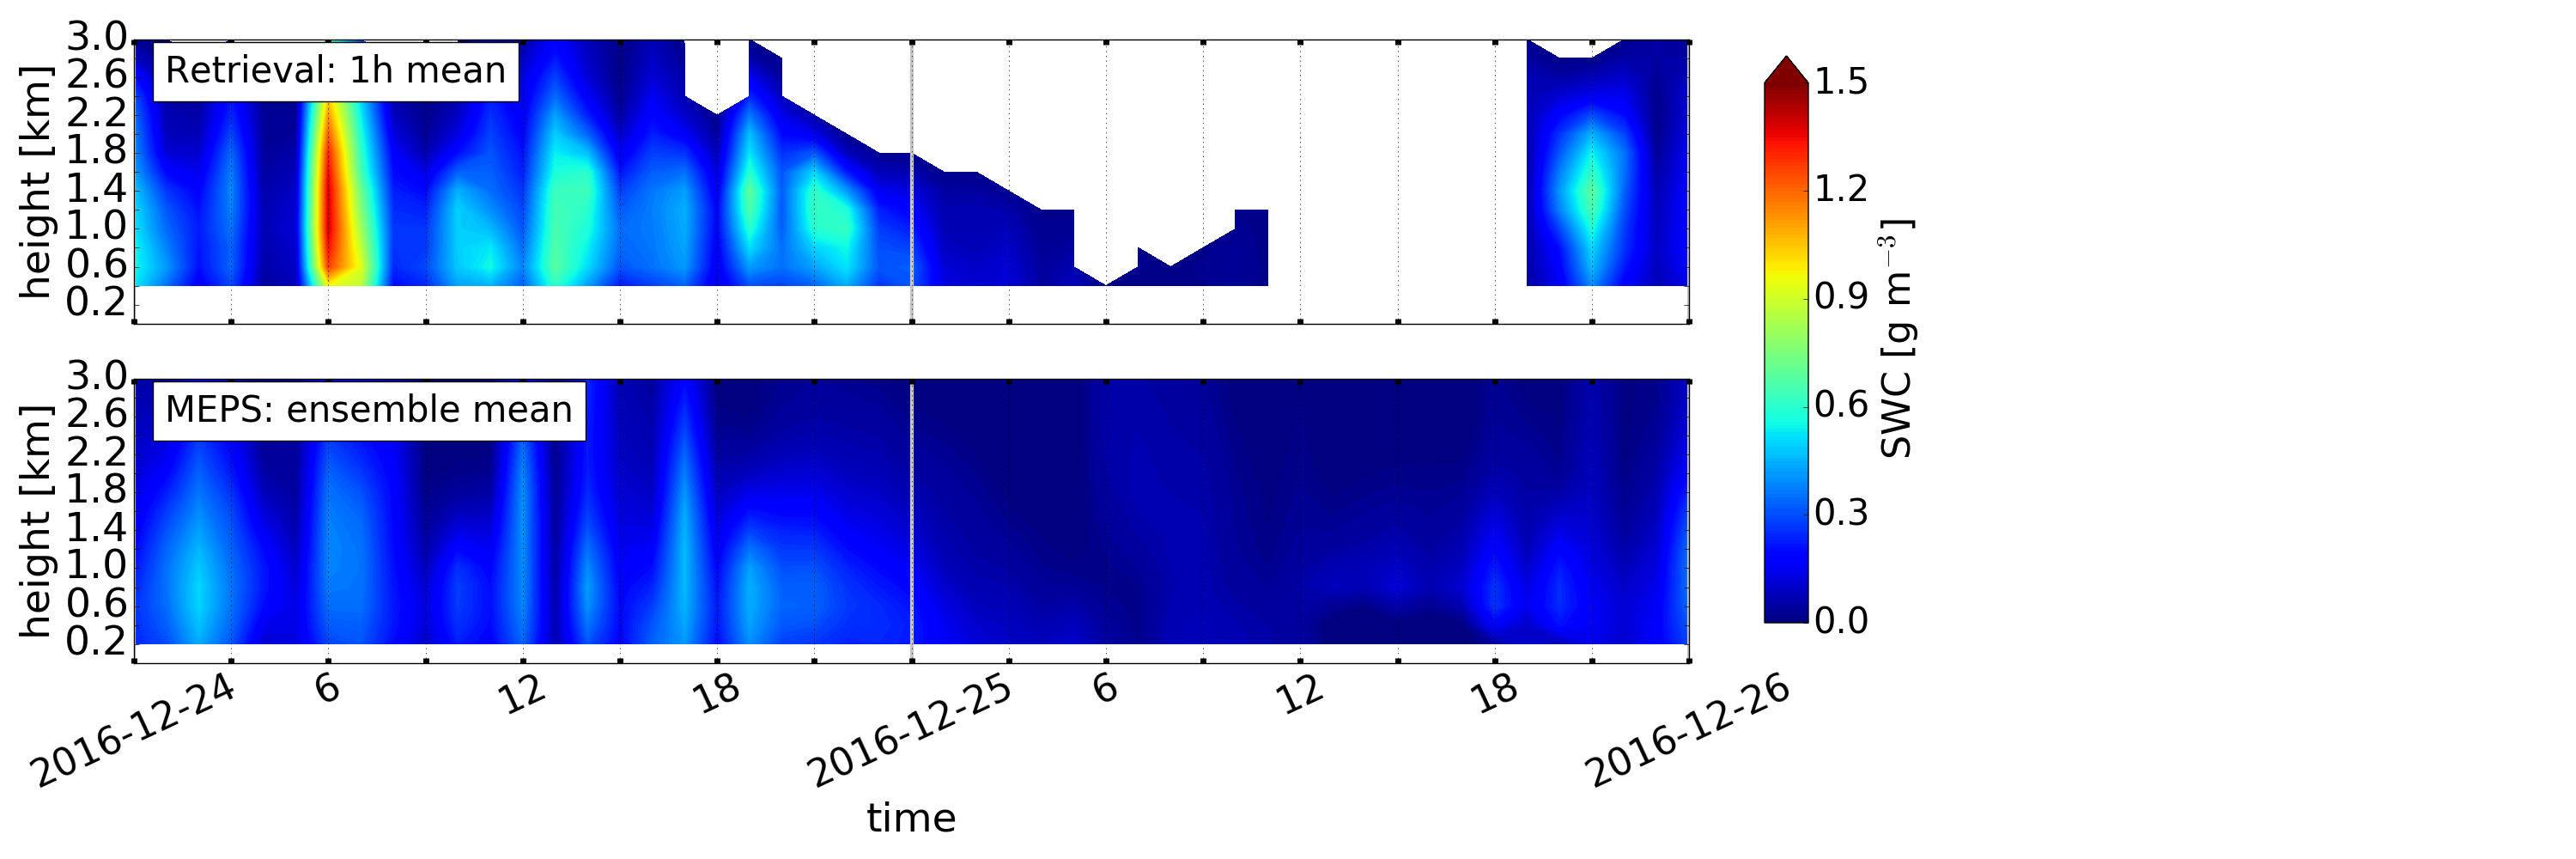
\includegraphics[trim={0.cm 2.2cm 19.cm 0.5cm},clip,width=0.9\textwidth]{./fig_vert_SWC_EM/20161224}
		\caption{}\label{fig:SWC_EM:24}
	\end{subfigure}
	% 3h
	\begin{subfigure}[t]{\textwidth}
		\centering
		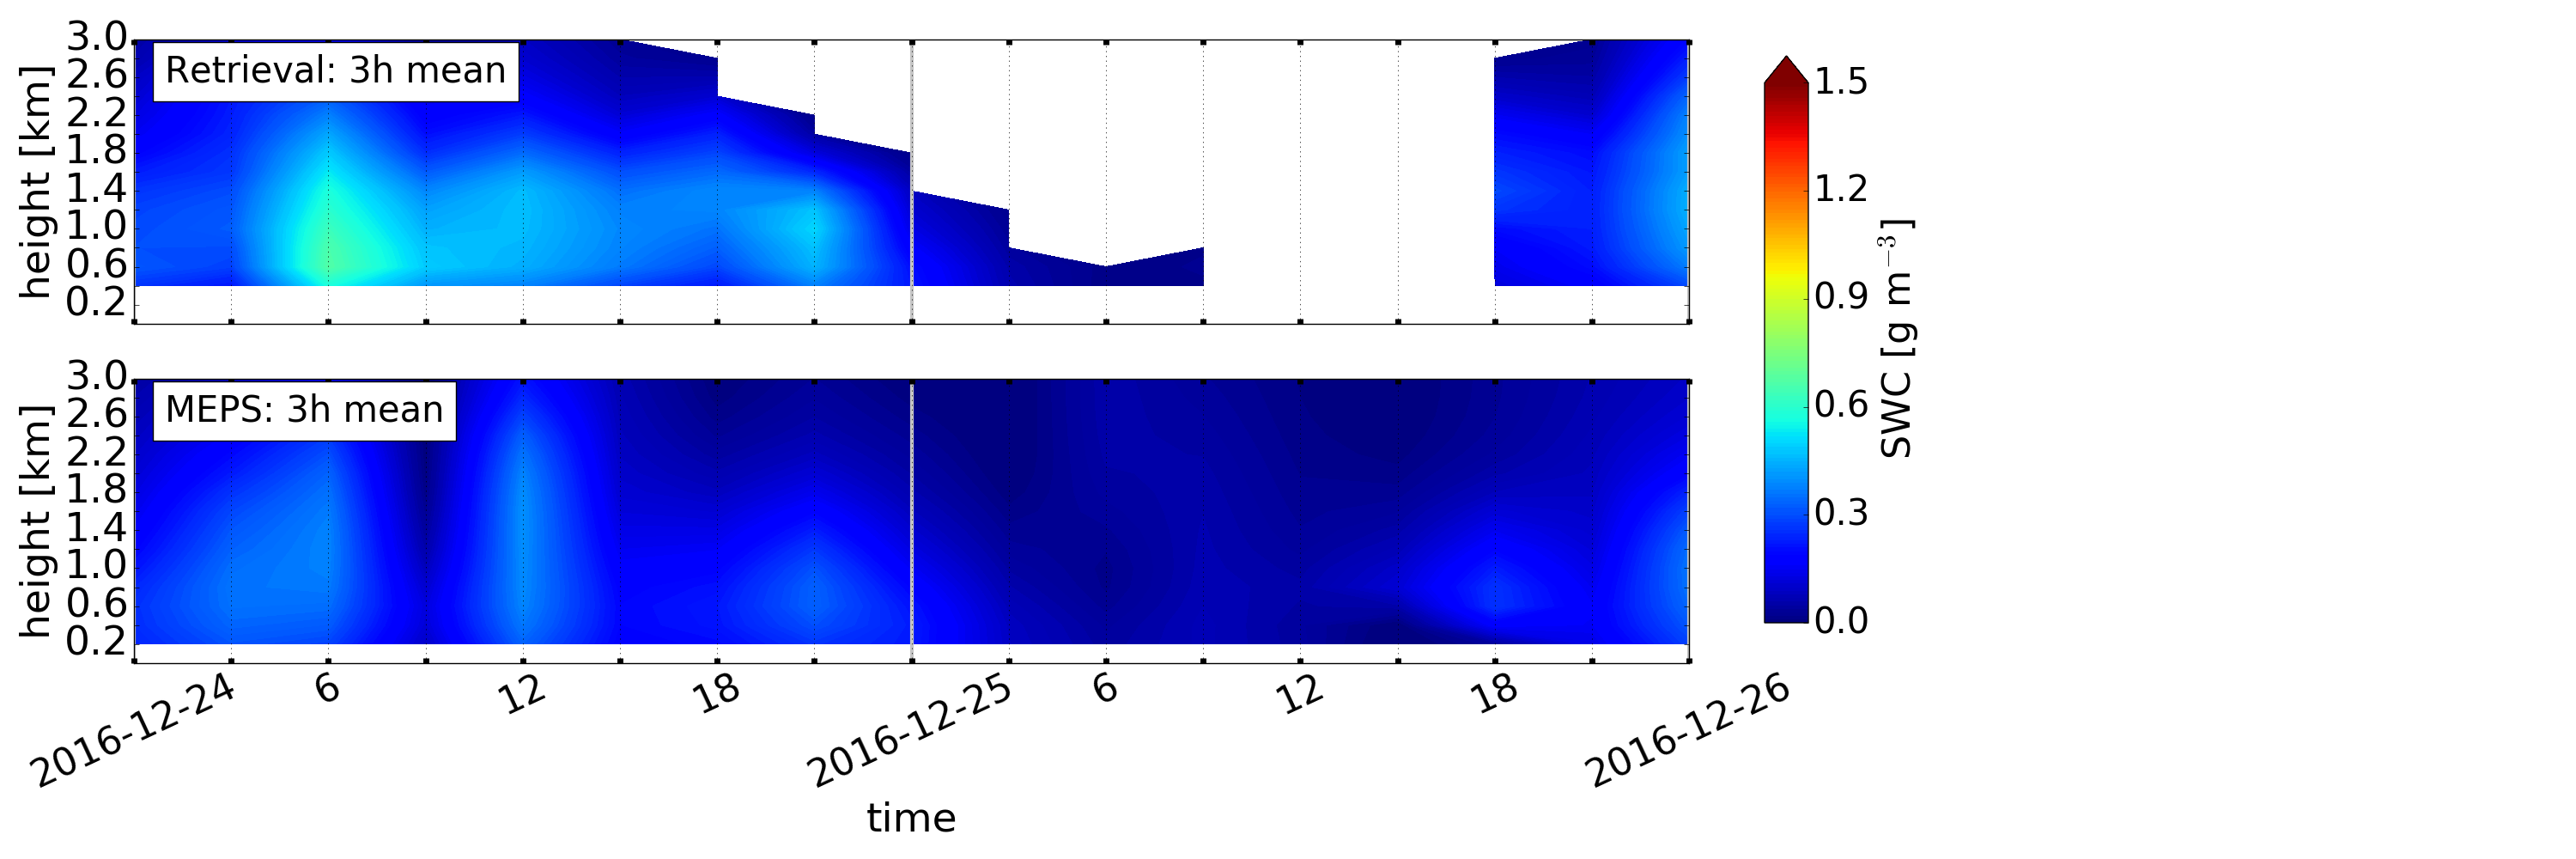
\includegraphics[trim={0.cm 0.8cm 19.cm 0.5cm},clip,width=0.9\textwidth]{./fig_vert_SWC_3h/20161224}
		\caption{}\label{fig:SWC3h:24}
	\end{subfigure}
	\caption{\textit{(Continued from previous page.)} Initialisation \SI{26}{\dec}.}
\end{figure}
%%%%%%%%%%%%%%%%%%%%%%%%%%%%%%%%%%%%%%%%%%%%%%
\noindent
\Cref{sec:sfc_acc} describes the overestimation of surface snow accumulation during the intensification of the extreme storm. MEPS forecasted more ground accumulation than it was observed. One approach was to see, if the wind might have had an influence on the surface measurement of the double fence, which did not show to be true. A comparison of the hourly values of MEPS, shows that neither on \SI{24}{\dec} nor on \SI{25}{\dec} or \SI{26}{\dec} the vertical snow amount was higher than the observations (\Cref{fig:SWC_EM:24}, \ref{fig:SWC_EM:25}, and \subref{fig:SWC_EM:26}). \Cref{fig:EM09} shows very intense individual ensemble members, but no prominent sign of overestimation when the surface miscalculation was present. 
\\
During \SIrange{24}{26}{\dec} was the wind constantly from the west with higher wind speeds observed than during \SIrange{21}{23}{\dec} (\Cref{fig:res:sfc_wd23}, \subref{fig:res:sfc_wd25}, \subref{fig:res:sfc_wd26}; \Cref{fig:res:sfc_wd21}, \subref{fig:res:sfc_wd22}, \subref{fig:res:sfc_wd24}; \Cref{fig:res:sfc_ws23}, \subref{fig:res:sfc_ws25}, \subref{fig:res:sfc_ws26}, and \Cref{fig:res:sfc_ws21}, \subref{fig:res:sfc_ws22}, \subref{fig:res:sfc_ws24}). \Cref{fig:scat:wd2123} and \subref{fig:scat:wd2426} indicate a better agreement between the forecasted and observed wind directions when precipiation overestimation occurred. During \SIrange{24}{26}{\dec} were the observed wind speeds higher than on the previous days, and as \Cref{fig:scat:ws2123} and \subref{fig:scat:ws2426} present is the correlation between observation and forecasts lower during high wind speeds. The high wind speeds from the west followed a pulsing storm pattern with intense and less intense precipitation. The pulsing pattern is forecasted by MEPS for initialisations longer than \SI{24}{\hour} prior. Since the model gets the wind direction correctly and the affect of local mountains it follows that there seems to be some kind of interaction issue between the vertical snow amount and the surface accumulation. Vertical instantaneous values every hour can lead to a misinterpretation of the here presented results. 
%%%%%%% image variability %%%%%%%%%%%%%%%%
\begin{figure}[t!]
	\centering
	\begin{subfigure}[b]{\textwidth}
		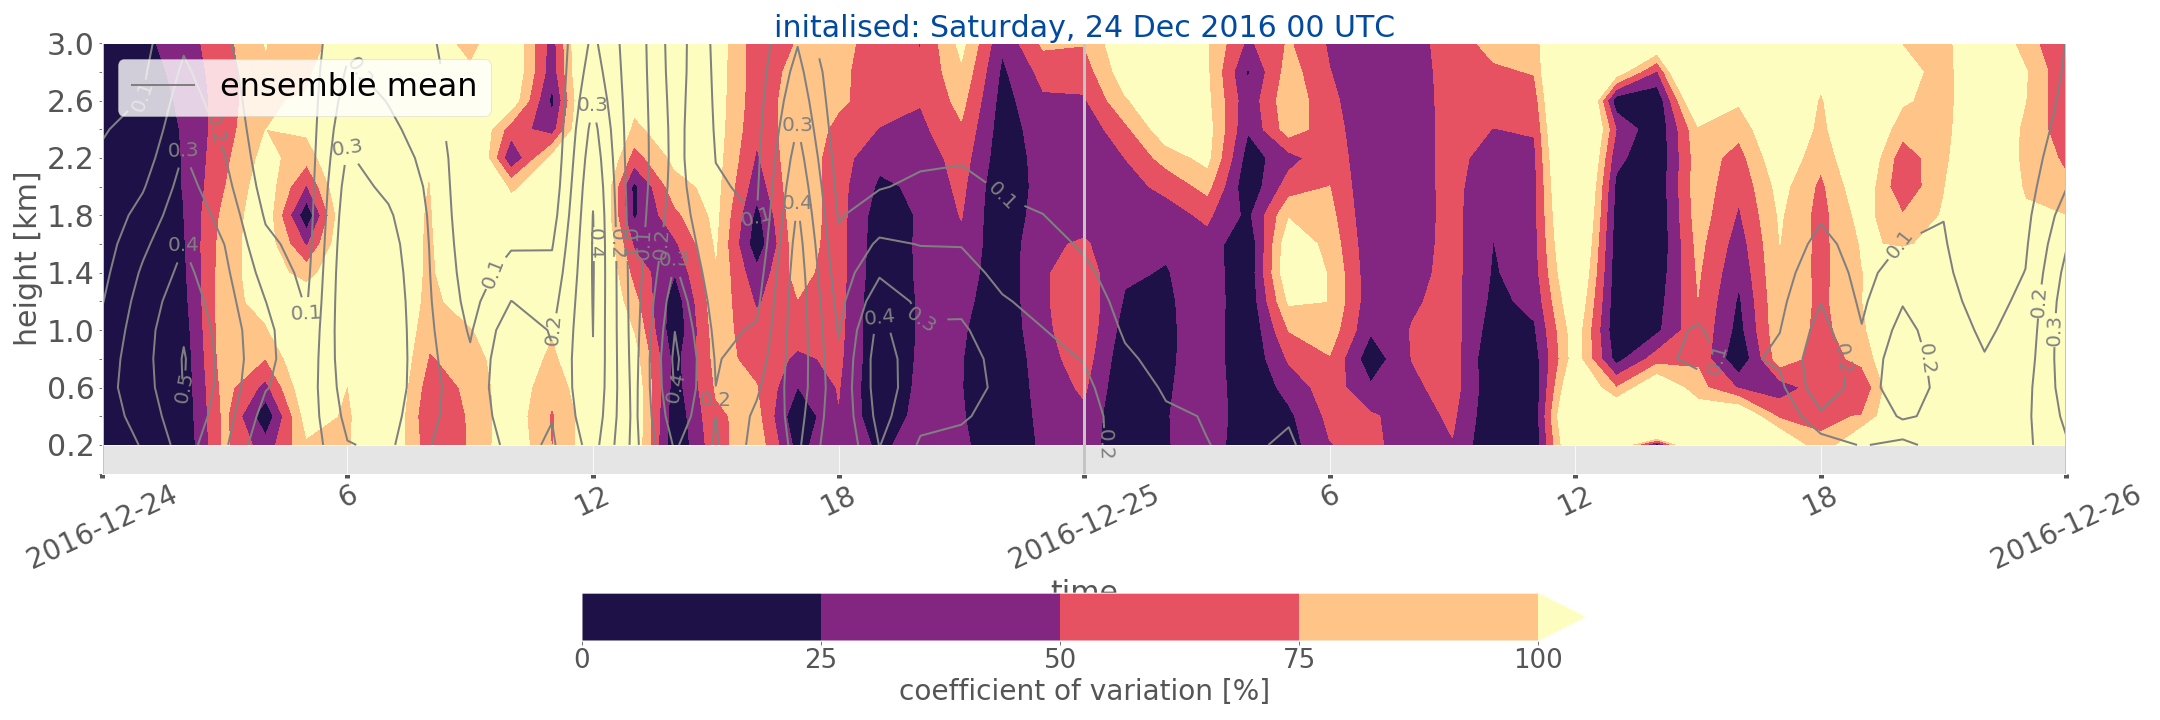
\includegraphics[trim={0cm 0cm 0cm 0cm},clip,width=\textwidth]{./fig_variation/20161224}
		\caption{}\label{fig:vari:EM24}
	\end{subfigure}
	\caption{SWC variation of the ten ensemble members of MEPS. The lighter the colour according to the colourbar the higher the variation between the perturbed ensemble members. In grey the ensemble mean of all ten members.}\label{fig:ens_vari24}
\end{figure}
%%%%%%%%%%%%%%%%%%%%%%%%%%%%%%%%%%%%%%%%%%%%%%
The ensemble variability in \Cref{fig:vari:EM24}, \Cref{fig:vari:EM25}, and \subref{fig:vari:EM26} show that the ensemble members are divided about the existence of the exact pulsing. 
\\
\\
While the wind direction of MEPS has a good agreement shows the wind speed larger values over all days. Although MEPS includes ten perturbed ensemble members the insufficiency of AROME-MetCoOp too high wind prediction in extreme situations is not resolved. The regional model wind prediction is still dependent on the intensity of the storm. As \cite{muller_arome-metcoop:_2017} also mentioned are higher wind speeds in general better forecasted in AROME-MetCoOp than in ECMWF. 
%%%%%%%%%%%%%%%%%%%%%%%%%%%%%%%%%%%%%%%%%%%%%%%%%%%%%%%%%%%%%%%%%%%%%%%%%%
\section{Discussion all}
\textcolor{red}{This section needs another title! Just collecting up-coming disscussion points}
Of course, more storms should be investigated to find the exact correlation between the surface observations and the estimated accumulation to see if the deviation keeps as small for different snow patterns at Haukeliseter. 
